% Can a bank's disclosed diversification effect be reproduced from public data?
% Evidence from ten years of Goldman Sachs Value-at-Risk disclosures.
%
% Title form follows the author's previous working paper: a question, then an
% "Evidence from" subtitle, with the running head a short gerund phrase.
%
% Layout follows the author's previous working paper: 11pt letterpaper article,
% 1in margins, newtx (Times), running head, booktabs tables with a note block
% under each. That paper departed from its own predecessor by moving to APA
% author-date; this one inherits the departure rather than repeating it, so
% apacite is carried over unchanged.
%
% Build: latexmk -pdf main.tex   (pdflatex + bibtex; biber is not required)

\documentclass[11pt,letterpaper]{article}
\usepackage[margin=1in,headheight=14pt]{geometry}
\usepackage[T1]{fontenc}
\usepackage[utf8]{inputenc}
\usepackage{amsmath,amsthm}
\usepackage{newtxtext,newtxmath}
\usepackage{microtype}
\usepackage{graphicx,booktabs,tabularx,array,multirow}
\usepackage{caption}
\usepackage{enumitem}
\usepackage{setspace}

\usepackage[natbibapa]{apacite}

\usepackage{xurl}
\usepackage[hidelinks]{hyperref}
% Carried from the previous paper, where a justified line containing the
% repository URL opened a gap at its hyphen. The glue is removed and the break
% points restricted to separators no reader would mistake for address
% characters. Both have to be set after xurl's own begin-document hook.
\AtBeginDocument{%
  \Urlmuskip=0mu plus 0mu%
  \def\UrlBreaks{\do\/\do\.\do\=\do\?\do\&\do\_}%
  \def\UrlBigBreaks{\do\:}}
\usepackage{fancyhdr}
\usepackage{placeins}
\usepackage{etoolbox}

\providecommand{\SohamLocation}{\textit{India}}

\hypersetup{%
  pdftitle={Can a bank's disclosed diversification effect be reproduced from
            public data? Evidence from ten years of Goldman Sachs
            Value-at-Risk disclosures},
  pdfauthor={Soham Abhay Parundekar},
  pdfsubject={Independent replication of Goldman Sachs's disclosed
              Value-at-Risk diversification effect from public data},
  pdfkeywords={Value-at-Risk, diversification effect, risk disclosure,
               historical simulation, backtesting, 10-K}}

\setstretch{1.06}
\setlength{\parindent}{1em}
\setlength{\parskip}{3pt}
\setlength{\emergencystretch}{2em}
\clubpenalty=10000
\widowpenalty=10000
\setlength{\textfloatsep}{13pt plus 3pt minus 3pt}
\setlength{\floatsep}{11pt plus 2pt minus 2pt}
\captionsetup{font=small,labelfont=bf,labelsep=period,justification=raggedright,
              singlelinecheck=false,skip=7pt}
\setcounter{topnumber}{2}
\setcounter{totalnumber}{3}
\renewcommand{\topfraction}{0.90}
\renewcommand{\textfraction}{0.08}
\renewcommand{\floatpagefraction}{0.80}

\pagestyle{fancy}
\fancyhf{}
\fancyhead[L]{\footnotesize Reproducing a disclosed diversification effect}
\fancyfoot[C]{\thepage}
\renewcommand{\headrulewidth}{0.25pt}

\newcolumntype{Y}{>{\raggedright\arraybackslash}X}
\newcommand{\E}{\mathbb{E}}
\newcommand{\Var}{\operatorname{Var}}
\newcommand{\ind}{\mathbf{1}}
\newcommand{\F}{\mathcal{F}}
% Objects specific to this paper. The previous paper's macros were for a
% worst-of payoff and an SVI surface and have no counterpart here.
\newcommand{\VaR}{\operatorname{VaR}}                 % the risk measure
\newcommand{\cat}{c}                                  % a risk category
\newcommand{\cats}{\mathcal{C}}                       % the four categories
\newcommand{\divef}{D}                                % diversification effect
\newcommand{\divpct}{d}                               % the same, as a share
\newcommand{\window}{W}                               % lookback window length
\newcommand{\cover}{\alpha}                           % coverage level
\newcommand{\notetext}[1]{\vspace{4pt}\par\noindent{\footnotesize\raggedright #1\par}}

\newtheorem{proposition}{Proposition}
\newtheorem{remark}{Remark}
\renewcommand{\arraystretch}{1.12}

\begin{document}

\thispagestyle{plain}
\begin{center}
{\LARGE\bfseries Can a bank's disclosed diversification effect\\
 be reproduced from public data?\par}
\vspace{7pt}
{\large Evidence from ten years of Goldman Sachs Value-at-Risk disclosures\par}
\vspace{14pt}

{\fontsize{10.1}{11.7}\selectfont\bfseries Soham Abhay Parundekar\par}
\vspace{1.5pt}
{\fontsize{8.0}{9.4}\selectfont\href{mailto:parundekarsoham@gmail.com}%
  {\nolinkurl{parundekarsoham@gmail.com}}\par}
\vspace{1.0pt}
{\fontsize{8.5}{10.0}\selectfont Independent Researcher, \SohamLocation\par}
\end{center}
\vspace{8pt}

\begin{abstract}
% Written last and revised after peer review. The earlier version quoted a
% regression trend whose p-value assumed an independence that overlapping
% five-year windows rule out, and described the amplitude comparison as an
% exact reproduction when ten observations cannot establish that. Both are
% restated here.
\noindent
Every large dealer reporting market risk under Item 7A publishes Value-at-Risk
by risk category and a single reconciling line between those categories and the
firmwide total. The category figures are levels. The reconciling line, the diversification
effect, is a relationship, and the relationship it reports is the one thing
the filing withholds. That asymmetry makes it the single disclosed quantity an
outside party can check. This paper tests it on ten consecutive Goldman Sachs filings,
fiscal years 2016 through 2025, with a historical-simulation engine run at the
bank's own disclosed settings --- full revaluation, a five-year scenario window
and age-weighted scenarios --- over a proxy book of seventeen public risk
factors sized to the disclosed split of risk across categories.

The level reproduces and the steadiness does not. Goldman's effect has averaged
42.0\% of summed category VaR with a year-to-year standard deviation of 2.08
percentage points; a book sized once and then left alone averages 41.6\%, which
no test on ten annual observations separates from the disclosure, with a
standard deviation of 6.33 ($F = 9.26$, $p = 0.003$). The firm's second
disclosed measure locates the failure. Period-end against period-end the two
amplitudes cannot be told apart; year on year the disclosed series carries
nothing forward (lag-1 autocorrelation $-0.47$) while the proxy carries almost
everything ($+0.9$). What fails to reproduce is not how far the ratio moves but
whether it comes back. Sweeping the undisclosed decay rate across
sixteen values, from equal weighting to a 6.6-day half-life, never brings the
proxy nearer than three times the disclosed steadiness, and the rates that best
repair the engine's coverage are among the worst on steadiness. Across all
sixteen sleeve-sign configurations, five match the disclosed steadiness and none
of those averages above 35.6\%, eight reach 40\% and the steadiest of those
varies by 3.68 points; none does both.

\end{abstract}

\noindent\textit{Keywords:} Value-at-Risk; diversification effect; risk
disclosure; historical simulation; backtesting.\par
\noindent\textit{JEL classification:} G21, G28, G32.
\vspace{8pt}

% Drafted against audit/outline.md §1. Every figure in this section is read
% from data/processed/diversification_comparison.csv,
% robustness_sign_variants.csv, robustness_windows.csv and
% robustness_age_weighting.csv in the frozen research repository; all four are
% hash-recorded in audit/evidence_freeze.csv at commit 1e6bdd74.

\section{Introduction}\label{sec:introduction}

Every large dealer that reports market risk under Item 7A of Form 10-K
publishes a table with roughly the same shape. Average daily Value-at-Risk is
broken out by risk category, the categories are added up, and a single negative
line is subtracted to arrive at the firmwide figure. Goldman Sachs calls that
line the diversification effect, and defines it as the difference between total
VaR and the sum of the VaRs of its four risk categories: interest rates, equity
prices, currency rates and commodity prices. Every other entry in the table is
a level. How much could be lost on rates, on equities, on currencies, on
commodities. The diversification line is not a level. It is the only number in
the table that depends on how those four exposures move against one another,
and co-movement is the one input the filing never publishes.

That asymmetry is what makes the line testable from outside, and it is also
what bounds any such test. A reader cannot check a disclosed interest-rate VaR
without knowing the rate book. A reader who builds a portfolio consistent with
the disclosed split of risk across categories, and exposes it to public market
data, can at least ask whether the co-movement that portfolio generates
resembles the co-movement the filing reports. That is the exercise here, and
the portfolio is a proxy throughout. It is calibrated so that each sleeve
carries the share of standalone risk that Goldman discloses for the
corresponding category; it is not a reconstruction of Goldman's positions, and
its dollar size is a normalisation that carries no information. What is being
tested is whether a static book with the disclosed risk structure, driven by
public factors, produces the disclosed diversification. Nothing in the paper
identifies a position, a desk, or a hedge.

The disclosures themselves make the test worth running, and they are more
specific about method than the VaR tables alone suggest.
\citet{jorion2002informative} showed that bank VaR disclosures are informative
about subsequent trading volatility, which is the premise any replication
presumes. The literature that followed has concentrated on the quality and the
conservatism of the reported numbers: \citet{perignon2010level} graded
disclosure practice across a cross-section of commercial banks,
\citet{perignon2008overstate} asked whether the levels banks report are
systematically too high, and \citet{perignon2010diversification} examined the
diversification component directly, on quarterly observations for four US banks
running to the first quarter of 2007. Those studies work across institutions,
and at the reporting frequency their data allow.

This paper adds three things to that base. The first is a single-dealer series
long enough to contain regime breaks rather than straddle one. Goldman's
diversification effect is reconstructed from ten consecutive filings covering
fiscal years 2016 through 2025, a decade that includes the March 2020
dislocation and the 2022--2023 tightening cycle. The second is a replication
run at the bank's own disclosed settings. Every filing in the sample states
that Goldman computes VaR by historical simulation with full valuation, samples
its scenarios from five years of historical data, and weights that data so that
the importance of older observations decays. All three are implemented here, on
seventeen factors drawn from the US Treasury and ECB curves and from
exchange-traded prices, with the interest-rate sleeve valued by full bond
revaluation rather than by a duration approximation. The engine is therefore
capable of disagreeing with the disclosure in a way that an identity built out
of the disclosed numbers cannot, and when it does disagree the disagreement
cannot be attributed to a cruder method. The third is a decomposition. Goldman discloses the same quantity twice, as an
annual average and as a period-end snapshot, and comparing each against its
proxy analogue separates how far the ratio moves from whether those movements
persist. The separation is what turns a failure to reproduce stability into a
specific claim about mean reversion, and it uses only what the filings already
publish. Running the complete space of sign configurations for the four sleeves
then bounds how closely a static book can match the level and the steadiness at
once, which turns out to be the binding constraint.

The disclosed series is remarkably flat. Across the ten years the
diversification effect ranges from 39.0\% to 45.5\% of summed category VaR,
with a mean of 42.0\% and a standard deviation of 2.08 percentage points. A
regression on the year index finds no trend ($p = 0.23$). A decade containing a
pandemic, a zero-rate period and more than 500 basis points of policy
tightening moved the reported co-movement of Goldman's four risk categories by
about two points of standard deviation, and moved it in no particular
direction.

The replication reproduces that level and does not reproduce that steadiness.
At the disclosed five-year window, a book sized once on 2019 and then left
alone averages 41.6\% against the disclosed 42.0\%; the two levels are
statistically indistinguishable ($p = 0.84$). Its standard deviation across
those years is 6.33 percentage points against the disclosed 2.08, a difference
a variance-ratio test puts at $p = 0.0028$. And the two move differently over
the decade: Goldman's second-half mean sits 0.8 points above its first, while
the proxy's sits 8.5 points below.

Goldman's second disclosed measure of the same quantity says what kind of
failure it is. Alongside the average daily figure the filings give a period-end
snapshot, and that series has a standard deviation of 6.72 points: the firm's
diversification ratio moves a great deal, and what is steady is its mean over a
year rather than the ratio itself. Measured period-end against period-end the
proxy's variation is statistically indistinguishable from Goldman's. What
separates them is persistence. The lag-1 autocorrelation of consecutive annual
values is $-0.47$ for Goldman's average daily series and essentially zero for
its period-end series, against roughly $+0.9$ for both proxy series: Goldman's
movements do not carry forward and the proxy's do. What fails to transfer is
therefore not stability but mean reversion, and mean reversion is what the
disclosed steadiness consists of.

The natural objection is that a proxy book on seventeen factors is simply a
blunter instrument than the bank's, and that the gap measures the crudeness of
the replication. Adopting Goldman's disclosed age weighting tests that
objection directly, and refutes it. Weighting the scenario set toward recent
observations raises the year-to-year standard deviation from 6.33 to between
9.46 and 10.04 points, four to five times the disclosed figure, across decay
rates with half-lives of three weeks and three months. It does so while making
the engine a demonstrably better risk model: the exception rate falls from
6.98\% to 5.45\% against a nominal 5\%, and the Kupiec proportion-of-failures
test moves from rejecting the model below any conventional level to a $p$-value
of 0.328. The disclosed weighting is the correct specification, the filings say
so, and applying it widens the stability gap rather than closing it.

Nor is the gap an artefact of one calibration of the sleeves. The four can be
signed in sixteen ways and all sixteen were run. Taking the disclosed standard
deviation itself as the bar, five configurations are at least that steady and
the highest of those averages 35.64\%, six points below the disclosure; eight
average 40\% or more and the steadiest of those varies by 3.68 points a year.
No configuration achieves both. Within this engine the two properties of the
disclosed series trade off against each other, and that frontier, rather than
any single calibration, is the paper's central result. It also points at what a
static book omits. A dealer that reprices positions daily, and whose hedges
respond to the correlations it observes, can hold a diversification ratio
steady in a way that a fixed portfolio exposed to the same market cannot.
Goldman's own filings attribute its year-over-year VaR changes to exposure
movements as well as to volatility in four consecutive years.

The remainder of the paper is organised as follows. Section~\ref{sec:disclosed}
sets out what Goldman discloses, how the series was extracted from the filings,
and where this exercise sits relative to prior work.
Section~\ref{sec:sample} describes the factor panel and the choices that shaped
it. Section~\ref{sec:method} specifies the historical-simulation engine, the
disclosed settings it adopts, and the calibration that ties the proxy book to
the disclosed split. Section~\ref{sec:validation} reports the validation:
unit-level checks, independent reproduction of the backtest statistics, and the
formal coverage tests applied to the engine's own output.
Section~\ref{sec:results} presents the comparison against the disclosures and
Section~\ref{sec:assumptions} isolates which assumptions the stability result
depends on. Section~\ref{sec:limitations} states what the exercise cannot
establish, and Section~\ref{sec:conclusion} concludes. Code, extracted
disclosures and model output are available in the repository cited in the data
availability statement.

% Drafted against audit/outline.md §2. Disclosure figures and the identity
% check come from data/processed/gs_var_average_daily.csv; Goldman's own
% wording is quoted from references/sec_filings/, both hash-recorded in
% audit/evidence_freeze.csv at commit 1e6bdd74.
%
% Two corrections to the outline's prior-work summary, made at drafting time
% against the source register: Pérignon, Deng and Wang (2008) study six
% Canadian banks, not US ones, and their abstract attributes the overstatement
% they find partly to underestimated diversification, which makes them closer
% to this paper's subject than the outline implied.

\section{The disclosed diversification effect, and prior work}\label{sec:disclosed}

\subsection{What Goldman discloses, and how the effect is defined}

The definition is Goldman's own, and it is worth quoting because the whole
exercise depends on it. In the words of the FY2025 filing, the "[d]iversification
effect in the tables below represents the difference between total VaR and the
sum of the VaR for the four risk categories," and "[t]his effect arises because
the four market risk categories are not perfectly correlated"
\citep{gs10k}. The four categories are interest rates, equity prices, currency
rates and commodity prices. The measure is a one-day 95\% VaR, and the filings
state that a single model produces both the category figures and the total,
which matters here: the diversification effect is internal to one model run
rather than the residual of aggregating four separate ones.

Table~\ref{tab:disclosed} gives the series. Across the ten fiscal years the
effect has sat between 39.0\% and 45.5\% of summed category VaR, averaging
42.0\% with a standard deviation of 2.08 percentage points and no discernible
trend. The dollar figures underneath it move a great deal: summed category VaR
runs from \$89 million in 2017 to \$209 million in 2022, and total VaR from
\$54 million to \$114 million over the same two years. The ratio of the two
barely moves.

% Generated by build/make_tables.py from gs_var_average_daily.csv. Do not edit.

\begin{table}[tbp]
\centering
\caption{Goldman Sachs average daily Value-at-Risk by risk category, and the disclosed diversification effect, FY2016--FY2025}
\label{tab:disclosed}
\begin{tabular}{@{}lrrrrrrrr@{}}
\toprule
 & \multicolumn{4}{c}{Risk category} & & & & \\
\cmidrule(lr){2-5}
Year & Rates & Equities & FX & Commod. & Summed & Diversif. & Total & \% of sum \\
\midrule
2016 & 45 & 25 & 21 & 17 & 108 & -45 & 63 & 41.7 \\
2017 & 40 & 24 & 12 & 13 & 89 & -35 & 54 & 39.3 \\
2018 & 46 & 31 & 14 & 11 & 102 & -42 & 60 & 41.2 \\
2019 & 46 & 27 & 11 & 12 & 96 & -40 & 56 & 41.7 \\
2020 & 71 & 55 & 23 & 20 & 169 & -75 & 94 & 44.4 \\
2021 & 60 & 43 & 13 & 25 & 141 & -55 & 86 & 39.0 \\
2022 & 97 & 33 & 32 & 47 & 209 & -95 & 114 & 45.5 \\
2023 & 96 & 29 & 24 & 19 & 168 & -69 & 99 & 41.1 \\
2024 & 81 & 37 & 26 & 19 & 163 & -71 & 92 & 43.6 \\
2025 & 70 & 47 & 24 & 17 & 158 & -68 & 90 & 43.0 \\
\bottomrule
\end{tabular}
\notetext{In millions of US dollars, except the final column. Average daily 95\% one-day Value-at-Risk as reported in the Market Risk Management section of each fiscal year's Form 10-K, taken from the filing that first reported the year rather than from a later filing's restatement. \emph{Summed} is the sum of the four category figures and is not itself disclosed. The diversification effect is disclosed as a negative number and reproduced with its sign; the final column expresses its magnitude as a percentage of the summed categories. Total VaR equals the summed categories plus the diversification effect in every year, exactly. The percentage averages 42.0 with a standard deviation of 2.08 across the ten years.}
\end{table}


The filings are also more specific about method than the tables alone suggest,
and three of those specifics are load-bearing later. Goldman states that it
uses "historical simulations with full valuation of market factors at the
position level by simultaneously shocking the relevant market factors for that
position"; that it samples "from five years of historical data to generate the
scenarios"; and that "[t]he historical data is weighted so that the relative
importance of the data reduces over time," which "gives greater importance to
more recent observations and reflects current asset volatilities"
\citep{gs10k}. The FY2016 and FY2017 filings put the factor count at
approximately 70,000; later filings drop the number. Section~\ref{sec:method}
adopts the method, the window and the weighting scheme; the decay rate is the
one piece of the description the filings leave unquantified.

One consequence of the weighting is stated in the filings explicitly: "even if
our positions included in VaR were unchanged, our VaR would increase with
increasing market volatility and vice versa" \citep{gs10k}. The disclosed
measure is therefore expected to respond to volatility without any change in
exposure, which is the behaviour a static replication can in principle
reproduce. What a static replication cannot reproduce is a change in exposure,
and Section~\ref{sec:results} shows that the filings attribute much of the
year-over-year movement to exactly that.

\subsection{Where the number comes from}

The figures are read out of the Market Risk Management section of each Form
10-K, filed under CIK 0000886982, for fiscal years 2016 through 2025. None of
it is available as structured data: the Item 7A tables carry no XBRL tagging,
so the numbers exist only as HTML table cells, and the cell layout is not
stable across filings. Six tables are extracted from each filing where
present: average daily VaR by category, period-end VaR, the year's high and low
by category, the daily net revenue distribution, and the exception counts at
the 95\% risk-management measure and the 99\% regulatory one. Appendix A gives
the full extracted series and the accession number of every filing.

Two features of the disclosures do the work of validating that extraction.

The first is an identity. Total VaR must equal the sum of the four categories
plus the diversification effect, because that is how the effect is defined. It
is therefore a property of a correct parse rather than a finding, and it is a
sharp one: a misread digit, a dropped minus sign or a column misalignment
breaks it. Across every average-daily row extracted --- 22 rows, since each
filing restates the prior year, covering 12 distinct disclosure years from 2014
to 2025 --- the residual is exactly zero. Net revenue bucket counts likewise sum
to the stated annual totals in all fourteen year-filing pairs that report them.

The second is redundancy. Because each filing restates the preceding year,
most years appear twice under different source filings, and the two readings
agree everywhere but once. The FY2023 filing reports 2022 average daily VaR as
\$113 million total against \$210 million summed, where the FY2022 filing had
reported \$114 million against \$209 million. The filing explains the change:
during the first quarter of 2023 Goldman added the currency exposure on certain
debt and equity positions to VaR, removed certain other positions, and
conformed the prior period. Both readings satisfy the identity, which is what
identifies this as a change in the measure's scope rather than a correction of
an error. Figures used throughout this paper are as first reported, so that a
methodology change does not sit inside the time series.

Disclosure practice is not perfectly stable either. The 99\% regulatory
exception count appears in eight of the ten filings but not in the FY2022 or
FY2023 filings, which report the 95\% count alone. Nothing in this paper
depends on the missing rows, but they are a reminder that what can be
reconstructed from disclosure is determined by the filer rather than the
researcher.

\subsection{Prior work}

The premise that these disclosures carry information is
\citet{jorion2002informative}'s: reported VaR predicts the variability of
subsequent trading revenue. What followed has largely asked how good the
reported numbers are.

Two findings recur. The first is conservatism.
\citet{perignon2008overstate} study six Canadian banks on daily data from 1999
to 2005 and find systematic overstatement, two exceptions in 7,354 trading
days against 74 expected at 99\%, which they attribute partly to banks
underestimating the diversification effect when aggregating across risk
categories. \citet{perignon2010level} construct a disclosure-quality index over
1996 to 2005 and report that historical simulation is by far the most common
method in practice, and that VaR computed that way carries very little
information about future volatility. The second is that bank VaR adapts slowly.
\citet{obrien2017evaluation} find that exceedances at large US banks were
excessive and clustered during the financial crisis, that a GARCH-based
benchmark achieved lower exceedance rates without clustering, and that variance
decompositions show limited ability of bank VaR methodologies to adjust to
crisis conditions. \citet{campbell2022australia} report the same shape in
Australia, with VaR too high in quiet periods and too low in stressed ones.

\citet{perignon2010diversification} is the nearest neighbour to this paper. It
tests whether banks underaccount for diversification across broad risk
categories, on quarterly observations for four US banks running to the first
quarter of 2007, and finds no systematic underestimation: disclosed
diversification effects are close to, and often larger than, the authors' own
estimates. The level result in Section~\ref{sec:results} corroborates that on a
different bank, a different period and a different method, and it should be read
as corroboration rather than discovery. Its sample ends before the financial
crisis and is quarterly, which leaves the behaviour of a disclosed
diversification effect across regime breaks as something a longer single-dealer
series can speak to.

\citet{danielsson2016modelrisk} supply the mechanism this paper's central
result turns on. They show that model risk, the potential for different
models to give inconsistent outcomes, rises with market uncertainty:
candidate models agree in calm periods and diverge significantly in distress.
Their object is risk forecasts in general rather than a disclosed
diversification ratio, but the diversification effect is a function of a
correlation structure estimated from data, and the finding here is a reading of
their result through that one statistic. Where their models diverge from each
other, a reconstruction diverges from the thing it reconstructs.

Finally, the methodological literature this paper borrows from directly is
small and is introduced where it is used:
\citet{kupiec1995} and \citet{christoffersen1998} for the coverage tests,
\citet{bcbs1996backtesting} for the supervisory zones,
\citet{boudoukh1998hybrid} for the age-weighted quantile that implements
Goldman's disclosed weighting, and \citet{hullwhite1998} with
\citet{riskmetrics1996} for the volatility-weighted variant.

% Drafted against audit/outline.md §3, with one deviation: the outline listed
% the 2022 restatement here as well as in §2. It is covered in §2.2 and is
% cross-referenced rather than repeated. §3.2 instead explains where the
% sample boundaries come from, which the outline left implicit.
%
% Figures from data/processed/gs_filing_manifest.csv, factor_move_summary.csv
% and factor_moves.csv, hash-recorded in audit/evidence_freeze.csv at commit
% 716ecf4c.

\section{Sample and data}\label{sec:sample}

\subsection{Why one dealer over ten years}

A cross-section of banks and a single bank over a long period answer different
questions. A cross-section can establish how disclosure practice varies, which
is what \citet{perignon2010level} and \citet{campbell2022australia} do. A long
single-dealer series can ask whether one firm's reported co-movement holds up
across a change of regime, which needs the regime change inside the sample
rather than at its edge.

That is the trade this paper makes. One filer, ten consecutive fiscal years,
and enough of them that the sample contains the March 2020 dislocation, the
zero-rate period that followed, and the tightening cycle of 2022 and 2023. The
cost is that nothing here generalises to other banks: Goldman's disclosed
diversification effect is a fact about Goldman, and the stability this paper
fails to reproduce may be particular to its book. What is tested is a
reproduction, not a cross-sectional regularity.

\subsection{The sample, and where its boundaries come from}

The disclosures are the ten Form 10-K filings of The Goldman Sachs Group, Inc.,
CIK 0000886982, covering fiscal years 2016 through 2025 and filed between
February 2017 and February 2026. Appendix~\ref{sec:appendix_a} lists the
accession number, filing date and retrieval URL of each.

Both sample boundaries follow from one rule, stated in
Section~\ref{sec:disclosed}: every figure is taken from the filing that first
reported it, rather than from a later filing's restatement of it. Each 10-K
restates the prior year, so the FY2016 filing does carry 2014 and 2015 figures,
but only as comparatives. Reaching those years as first reported would
require the FY2014 and FY2015 filings, which are not in the sample because the
ten-year window was fixed before the as-first-reported rule made their absence
binding. Extending the series backwards is therefore a matter of fetching two
more filings rather than a limitation of method, and it was not done. At the recent end, FY2025 is
simply the most recent filing available at the retrieval date of 9 October
2026.

The factor panel's start date is set by the disclosed window rather than
chosen. A five-year lookback needs five years of scenarios before the first
valuation date, and the aligned trading calendar described below discards about
9\% of days, so five years of scenarios needs closer to six calendar years of
history. The panel begins on 5 January 2010 and runs to 30 December 2025,
3,670 aligned days, which leaves 1,376 days of history before the first
valuation date against the 1,260 the window consumes. One restatement in the
disclosed series is discussed in Section~\ref{sec:disclosed} and is not
repeated here; the figures used throughout are as first reported.

\subsection{The seventeen factors}

Table~\ref{tab:factors} lists the risk factors and Table~\ref{tab:factorstats}
summarises their daily moves. All seventeen come from the issuer of the
instrument, a central bank, or an exchange close: the US Treasury par yield
curve at two, five, ten and thirty years \citep{treasurycurve}; the European
Central Bank's euro area AAA central government spot curve at two, five and ten
years \citep{ecbcurve}; four equity indices; three currency pairs; and three
commodity funds. They are grouped to match Goldman's four disclosed categories
so that each sleeve can be sized against the corresponding disclosed share.

% Generated by build/make_tables.py from factor_move_summary.csv. Do not edit.

\begin{table}[tbp]
\centering
\small
\caption{The seventeen risk factors, grouped to match Goldman's four disclosed risk categories}
\label{tab:factors}
\begin{tabular}{@{}lllll@{}}
\toprule
Factor & Category & Instrument & Unit of daily move & Source \\
\midrule
us\_2y & Interest rates & Par coupon bond, semiannual & Yield change (pp) & US Treasury \\
us\_5y & Interest rates & Par coupon bond, semiannual & Yield change (pp) & US Treasury \\
us\_10y & Interest rates & Par coupon bond, semiannual & Yield change (pp) & US Treasury \\
us\_30y & Interest rates & Par coupon bond, semiannual & Yield change (pp) & US Treasury \\
eur\_2y & Interest rates & Zero-coupon bond, annual & Yield change (pp) & ECB \\
eur\_5y & Interest rates & Zero-coupon bond, annual & Yield change (pp) & ECB \\
eur\_10y & Interest rates & Zero-coupon bond, annual & Yield change (pp) & ECB \\
\addlinespace
equity\_us & Equity prices & S\&P 500 index & Fractional return & Exchange \\
equity\_europe & Equity prices & EURO STOXX 50 index & Fractional return & Exchange \\
equity\_japan & Equity prices & Nikkei 225 index & Fractional return & Exchange \\
equity\_em & Equity prices & Emerging-markets equity fund & Fractional return & Exchange \\
\addlinespace
fx\_eurusd & Currency rates & EUR/USD spot & Fractional return & Exchange \\
fx\_usdjpy & Currency rates & USD/JPY spot & Fractional return & Exchange \\
fx\_gbpusd & Currency rates & GBP/USD spot & Fractional return & Exchange \\
\addlinespace
commodity\_gold & Commodity prices & Gold fund & Fractional return & Exchange \\
commodity\_oil & Commodity prices & Crude oil fund & Fractional return & Exchange \\
commodity\_base\_metals & Commodity prices & Base metals fund & Fractional return & Exchange \\
\bottomrule
\end{tabular}
\notetext{Rate factors are repriced by full revaluation, which needs the level as well as the change, because the same 25 basis point move is worth a different amount of money at a 0.5\% yield than at a 5\% one. A yield change of 0.25 means 25 basis points throughout. Equity indices enter in local currency, so that currency risk stays in the currency sleeve rather than being counted twice. Commodities enter through exchange-traded funds rather than front-month futures; Section~\ref{sec:sample} gives the reason.}
\end{table}


% Generated by build/make_tables.py from factor_move_summary.csv. Do not edit.

\begin{table}[tbp]
\centering
\small
\caption{Daily moves by factor, 2010--2025}
\label{tab:factorstats}
\begin{tabular}{@{}lrrrr@{}}
\toprule
Factor & Mean & Std.\ dev. & Minimum & Maximum \\
\midrule
us\_2y & +0.06 & 4.73 & -57.00 & +34.00 \\
us\_5y & +0.03 & 5.62 & -35.00 & +31.00 \\
us\_10y & +0.01 & 5.63 & -36.00 & +29.00 \\
us\_30y & +0.00 & 5.51 & -45.00 & +29.00 \\
eur\_2y & +0.02 & 3.80 & -43.47 & +36.57 \\
eur\_5y & -0.01 & 4.35 & -31.25 & +29.35 \\
eur\_10y & -0.02 & 4.55 & -26.46 & +24.01 \\
\addlinespace
equity\_us & +0.056 & 1.134 & -11.984 & +9.515 \\
equity\_europe & +0.026 & 1.311 & -12.401 & +10.348 \\
equity\_japan & +0.052 & 1.381 & -12.396 & +10.226 \\
equity\_em & +0.026 & 1.409 & -12.479 & +8.053 \\
\addlinespace
fx\_eurusd & -0.004 & 0.576 & -5.001 & +3.176 \\
fx\_usdjpy & +0.016 & 0.621 & -4.552 & +4.061 \\
fx\_gbpusd & -0.003 & 0.586 & -7.604 & +3.791 \\
\addlinespace
commodity\_gold & +0.041 & 1.043 & -8.781 & +5.984 \\
commodity\_oil & -0.014 & 2.325 & -25.315 & +16.667 \\
commodity\_base\_metals & +0.014 & 1.283 & -8.371 & +6.191 \\
\bottomrule
\end{tabular}
\notetext{Equity, currency and commodity factors in percent per day; interest-rate factors in basis points per day. The two blocks are not comparable with one another, which is why the engine sizes sleeves against disclosed risk shares rather than against notional. 3,670 aligned trading days from 5 January 2010 to 30 December 2025.}
\end{table}


Seventeen factors against the roughly 70,000 the FY2016 and FY2017 filings
describe is the single largest difference between this model and Goldman's, and
the direction of its effect is known: fewer independent sources of risk means
less diversification available, which biases the measured effect downward
relative to a book with a richer factor set. It is not quantifiable here, and
Section~\ref{sec:limitations} says so rather than estimating it.

The two blocks of Table~\ref{tab:factorstats} are in different units and are
not comparable with each other. That is not a presentational awkwardness but
the reason the engine sizes sleeves against disclosed risk shares rather than
against notional: a dollar of two-year Treasury and a dollar of crude oil fund
carry risks that differ by more than an order of magnitude, so matching
Goldman's category proportions requires matching risk, not money.
Section~\ref{sec:method} gives the calibration.

\subsection{Three choices that shaped the panel}

Each of these changes the numbers, so each is stated rather than left in the
code.

\emph{Equity indices enter in local currency.} A dollar investor holding the
Nikkei carries yen risk as well as Japanese equity risk. Goldman reports
currency risk as a category of its own, so converting the indices to dollars
would push currency risk into the equity sleeve and count it twice, making the
category attribution --- the thing being matched --- meaningless.

\emph{Commodities enter through exchange-traded funds rather than front-month
futures.} On 20 April 2020 the NYMEX May 2020 WTI contract settled at
$-\$37.63$ per barrel, against a close of \$18.27 on 17 April
\citep{cftc2020wti}. A percentage return is not defined across a sign change,
and the implied one-day move of $-306\%$ is arithmetic rather than a price
movement a risk model should be asked to price. Funds cannot settle below zero.
The cost of the substitution is roll yield, which drags a fund away from spot
over long horizons; over one day it is second order, but it is a real
difference from a spot book and it is carried through to
Section~\ref{sec:limitations}.

\emph{Prices are adjusted for splits.} The crude oil fund used here ran a
one-for-eight reverse share split, effective after the close on 28 April 2020,
with post-split shares trading from the following day \citep{uso2020split}. On
unadjusted closes that is a 700\% overnight gain, and it would enter the
scenario set as a tail event in the middle of the most consequential stress
window in the sample, within days of the negative settlement above.
Split-adjusted closes are used throughout, for every traded instrument rather
than only this one.

\subsection{The trading calendar}

Tokyo, London, New York and the ECB keep different holidays, and the panel is
the intersection of their calendars rather than the union. Taking only days on
which every market traded costs about 9\% of trading days and leaves 225 to 233
observations a year against the 250 to 253 Goldman reports. The alternative,
forward-filling a closed market, would plant runs of exact zeros in the
scenario set and understate that factor's risk, which is a worse error than a
smaller sample: it would bias the thing being measured rather than merely
reducing the precision with which it is measured.

The reduced sample does cost power in every test reported in
Section~\ref{sec:validation}, and that is the price of the choice.

Two further properties of the panel are limitations rather than choices, and
neither is corrected. The surviving closes are still not simultaneous across
time zones, which depresses measured cross-market correlation and therefore
overstates diversification, in the opposite direction to the factor-count
bias above, which is why neither is used to argue the result one way or the
other. And the Treasury curve is quoted to the basis point, so at near-zero
policy rates the two-year yield shows no change at all on 21.1\% of days across
the panel, rising to 43.1\% of days in the second half of 2020. The build's
staleness check accommodates this by allowing longer runs of identical values
in yield factors than in traded prices; the longest unbroken run in the
two-year series is six days, against a limit of fifteen. The discretisation
slightly understates true rate variability through the near-zero years.

% Drafted against audit/outline.md §4, with one addition: a subsection
% specifying the age-weighted quantile. The outline predates the discovery
% that Goldman's disclosed weighting had never been implemented, so its
% bullets do not include it, and the estimator has to be defined formally
% before §7 can report the sweep that turns on it.
%
% Figures from data/processed/book_fixed_notionals.csv and config/params.yaml,
% hash-recorded in audit/evidence_freeze.csv at commit 1e6bdd74.

\section{Method}\label{sec:method}

\subsection{Instruments, and what full revaluation means here}

Equity, currency and commodity positions are linear in their factor: a one-day
fractional return on the factor is the fractional profit and loss on the
position. Interest-rate positions are not. They are repriced by discounting
their cashflows again at the shocked yield, which is what Goldman's phrase
``full valuation'' describes, rather than multiplied by a modified duration.

The two rate sub-sleeves keep their source's native convention. US positions
are par coupon bonds priced off the Treasury par yield curve with semiannual
coupons; euro positions are zero-coupon bonds priced off the ECB spot curve
with annual compounding. The alternative would be to convert one curve into the
other's convention, which needs a bootstrap the published data does not
support at these tenors. The cost of keeping both is that a dollar of euro zero
and a dollar of US par bond are not interchangeable: a zero has longer duration
than a par bond of the same maturity, so the sleeves differ per unit of
notional. The sizing described below targets risk rather than notional, which
absorbs the difference, but the instrument sets are not identical and
Section~\ref{sec:limitations} records that.

Writing $P(y, m)$ for the price of the relevant instrument at yield $y$ and
maturity $m$, the scenario return for a rate position under a historical yield
change $\Delta y_{s}$ observed on day $s$ is
\begin{equation}
r_{s} = \frac{P(y_{t} + \Delta y_{s},\, m)}{P(y_{t},\, m)} - 1 ,
\label{eq:revaluation}
\end{equation}
where $y_{t}$ is the yield at the close of the valuation date. The level enters
as well as the change, which is why the engine carries both: the same 25 basis
point move is worth a different amount of money at a 0.5\% yield than at a 5\%
one. Equation~\eqref{eq:revaluation} is also where convexity enters, and
Section~\ref{sec:assumptions} reports what it is worth by running the same
scenarios through the first-order approximation
$r_{s} \approx -D_{\mathrm{mod}}(y_{t}, m)\,\Delta y_{s}$ instead.

\subsection{Sizing within a sleeve, and sizing the sleeve against the disclosure}

Sizing happens in two stages, and only the second touches the disclosures.

Within a sleeve, instruments are weighted so that each contributes equal
standalone VaR over the calibration window. This is a neutrality choice rather
than an empirical claim: nothing is disclosed about the composition of
Goldman's rate book, so loading the sleeve onto any one tenor would be an
assumption with no support. Equal risk contribution is the weighting that
requires no such assumption.

The sleeve as a whole is then scaled so that its average daily VaR across the
calibration year equals the figure Goldman disclosed for that category. The
scaling is available in closed form, which is worth stating because it is the
design of the experiment rather than a computational convenience. Profit and
loss on every position here is proportional to its notional, so for a sleeve
$\cat$ with notionals $\mathbf{n}$ scaled by $k > 0$,
\begin{equation}
\VaR_{\cat}(k\mathbf{n}) = k \, \VaR_{\cat}(\mathbf{n}) ,
\label{eq:homogeneity}
\end{equation}
and the same proportionality carries through the average over the year. One
division per sleeve therefore lands exactly on the disclosed target.
Section~\ref{sec:validation} confirms that it does, to machine precision.

Equation~\eqref{eq:homogeneity} is positive homogeneity, which is one of the
four axioms \citet{artzner1999coherent} use to define a coherent risk measure
and one of the three VaR actually satisfies. It is worth naming because the
axiom VaR fails --- subadditivity --- is the subject of this paper's central
quantity, and the calibration leans on the one property that holds while the
experiment measures the one that does not.

The consequence is that the summed category VaR matches the disclosures by
construction and carries no information whatever. That is deliberate. Fixing
the four category figures leaves total VaR and hence the diversification effect
entirely free, because the total depends on how the four sleeves move together
and nothing in the calibration constrains that. Comparing the free quantity
against its disclosed counterpart is the experiment; the matched quantities are
the control.

Table~\ref{tab:book} gives the resulting book. Its dollar level is a
normalisation and should not be read as an estimate of anything: only the
ratios between sleeves carry meaning, and those come from the disclosures.

% Generated by build/make_tables.py from book_fixed_notionals.csv. Do not edit.

\begin{table}[tbp]
\centering
\small
\caption{The fixed proxy book after calibration to the FY2019 disclosed risk split}
\label{tab:book}
\begin{tabular}{@{}lllrr@{}}
\toprule
Factor & Category & Instrument & Maturity (y) & Notional (\$mm) \\
\midrule
us\_2y & Interest rates & Par coupon bond & 2 & 8,403 \\
us\_5y & Interest rates & Par coupon bond & 5 & 2,467 \\
us\_10y & Interest rates & Par coupon bond & 10 & 1,302 \\
us\_30y & Interest rates & Par coupon bond & 30 & 553 \\
eur\_2y & Interest rates & Zero-coupon bond & 2 & 18,162 \\
eur\_5y & Interest rates & Zero-coupon bond & 5 & 3,941 \\
eur\_10y & Interest rates & Zero-coupon bond & 10 & 1,427 \\
\addlinespace
equity\_us & Equity prices & Linear in factor & --- & 604 \\
equity\_europe & Equity prices & Linear in factor & --- & 478 \\
equity\_japan & Equity prices & Linear in factor & --- & 444 \\
equity\_em & Equity prices & Linear in factor & --- & 442 \\
\addlinespace
fx\_eurusd & Currency rates & Linear in factor & --- & 788 \\
fx\_usdjpy & Currency rates & Linear in factor & --- & 734 \\
fx\_gbpusd & Currency rates & Linear in factor & --- & 701 \\
\addlinespace
commodity\_gold & Commodity prices & Linear in factor & --- & 443 \\
commodity\_oil & Commodity prices & Linear in factor & --- & 165 \\
commodity\_base\_metals & Commodity prices & Linear in factor & --- & 341 \\
\bottomrule
\end{tabular}
\notetext{Notionals are the output of the sizing described in Section~\ref{sec:method}, not an estimate of anything Goldman holds. Sleeve totals are \$36,255mm of rates, \$1,968mm of equity, \$2,223mm of currency and \$949mm of commodity exposure, \$41,395mm in all. The rate sleeve dominates on notional and not on risk: a two-year note carries a fraction of the daily risk of a dollar of crude oil fund, which is the whole reason sizing targets risk rather than money. The dollar level is a normalisation and carries no information; only the ratios between sleeves do.}
\end{table}


\subsection{The engine and its timing convention}

For a valuation date $t$, the scenario set is the $\window$ most recent daily
factor moves up to and including $t$, applied to the book as it stands at the
market levels of $t$. Each scenario produces one profit-and-loss outcome per
sleeve and one for the book as a whole, and VaR is the loss at the
$\cover$ quantile of that distribution, reported as a positive number. Category
VaR uses only that category's positions. Total VaR moves every factor together,
historical day by historical day, which is what preserves the co-movement the
paper is testing. The diversification effect is
\begin{equation}
\divef_{t} = \VaR_{t}^{\text{total}} - \sum_{\cat \in \cats} \VaR_{t}^{\cat} ,
\qquad
\divpct_{t} = \frac{-\divef_{t}}{\sum_{\cat \in \cats} \VaR_{t}^{\cat}} ,
\label{eq:diversification}
\end{equation}
following Goldman's definition exactly, with $\divpct_{t}$ the share reported
throughout this paper.

The settings are the disclosed ones where the filings supply them:
$\window = 1{,}260$ trading days, which is the five years Goldman states it
samples from, and $\cover = 0.05$ for the 95\% risk-management measure. The
quantile is read off the finite scenario set by linear interpolation; the
discrete order statistic is the conservative alternative and
Section~\ref{sec:assumptions} reports the difference rather than assuming it
away. Appendix~\ref{sec:appendix_b} gives the reading conventions in full,
together with the argument behind the closed-form calibration and the
look-ahead probe.

The timing convention is stated explicitly because getting it wrong produces a
model that looks better than it is. VaR dated $t$ uses only the book, the
levels and the scenarios available at the close of $t$, and it is compared
against the profit and loss realised on $t+1$. No quantity dated $t+1$ enters
the VaR dated $t$. This is Goldman's own convention: the filings state that
daily net revenues are compared with VaR calculated as of the end of the prior
business day. Section~\ref{sec:validation} describes the test that
enforces it.

\subsection{Scenario age weighting}

Goldman states that its historical data is weighted so that the importance of
older observations decays. Implementing that replaces the equally weighted
quantile with a weighted one, following the hybrid approach of
\citet{boudoukh1998hybrid}. A scenario observed $k$ trading days before the
valuation date enters with weight
\begin{equation}
w_{k} = \frac{\lambda^{k}}{\sum_{j=0}^{\window-1} \lambda^{j}} ,
\qquad \lambda \in (0, 1] ,
\label{eq:ageweights}
\end{equation}
and VaR is read at the point where cumulative weight, rather than cumulative
count, reaches $\cover$. At $\lambda = 1$ every weight is $1/\window$ and the
estimator returns to the equally weighted percentile.

Two properties of the implementation matter for interpreting
Section~\ref{sec:assumptions}. The first is that the collapse at $\lambda = 1$
is exact, in both the interpolated and the discrete reading, which
Section~\ref{sec:validation} reports as a test: any difference between a
weighted and an unweighted run is therefore the weighting and not a change of
estimator. The second is that $\lambda$ is not disclosed. The filings describe
the scheme but not its rate, so the baseline keeps $\lambda = 1$, leaving no
undisclosed parameter inside it, and the rate is swept instead, at values
chosen for their half-lives rather than for how close they land to the
disclosures.

\subsection{Two books, and what each is for}

Two books are run, and conflating them would be a mistake.

The \emph{recalibrated} book is resized every year to that year's own disclosed
split. Its exposure mix tracks the disclosures exactly, which removes the
exposure mix from the comparison and leaves only the cross-category
correlations in the public data. It is the right book for asking whether the
diversification effect comes out where Goldman reports it. It is not a
forecast, and could not be: sizing the 2022 book uses a figure published in
February 2023.

The \emph{fixed} book is sized once, on 2019, and then left alone. Nothing
about it responds to anything disclosed afterwards, so the path its VaR takes
is driven purely by what happened to volatility and correlation. It is the
right book for the regime comparison, and the only defensible one for
backtesting, because its notionals were set before any of the data it is scored
on. 2019 is the base year because it is calm and precedes everything the
backtest scores, which makes 2020 onward out of sample with respect to sizing.

\subsection{The volatility-weighted variant}

One variant is run alongside the disclosed specification, because it addresses
a failure the disclosed specification has.
\citet{hullwhite1998} rescale each historical return by the ratio of today's
conditional volatility to the volatility in force when the return was observed,
so the scenario set is restated in current volatility units before the
percentile is taken. Volatility is estimated by exponentially weighted variance
with the \citet{riskmetrics1996} daily decay factor of 0.94, and the estimator
is causal by construction: the forecast stamped $t$ uses only moves up to $t$.
A GARCH(1,1) alternative is refitted each January on the history available at
that point.

Realised profit and loss always comes from the unscaled moves. What the book
actually made on $t+1$ is not a function of which model forecast it, and
scaling the outcome as well as the scenarios would make the backtest circular.

Age weighting and volatility weighting are easy to confuse and do different
things. Age weighting changes how much a scenario counts according to when it
happened. Volatility weighting changes the size of the scenario itself
according to the volatility regime it came from. Both turn out to repair the
engine's coverage, and neither repairs the diversification result, for a reason
Section~\ref{sec:assumptions} develops: both act on the scale of the scenario
set, and the diversification effect is a function of its correlation structure.

% Drafted against audit/outline.md §5. Three figures in that block were stale
% and are corrected here against the current suite and data: sizing error is
% 4.26e-14 percent rather than 6.6e-14, the Kupiec empirical size is 4.3% at
% the seed the test fixes rather than 4.8-5.8%, and the suite is 107 tests
% rather than 88. The outline records the corrections.
%
% Berkowitz and O'Brien (2002) is not cited: paywalled, never read, recorded
% as such in the source register.
%
% Evidence: data/processed/calibration_error_by_year.csv and the test suite,
% hash-recorded in audit/evidence_freeze.csv at commit 1e6bdd74.

\section{Validation}\label{sec:validation}

A model that runs is not a model that is right. Every check in this section
compares the engine against something outside it --- a hand calculation, an
independent implementation, a published boundary, an algebraic identity --- so
that agreement is evidence rather than self-report. The suite is 107 tests.
What none of it establishes is the resemblance between the proxy book and
Goldman's, and the last subsection says so plainly.

\subsection{The pricer against hand calculation}

The bond pricer is the one component where an error would be silent: a
mispriced bond produces a plausible VaR rather than an exception. A ten-year
bond with a 5\% semiannual coupon valued at a 6\% yield prices at
92.5612626, which the implementation reproduces to seven decimals, and it
trades below par because its coupon is a point under its yield. A zero-coupon
bond reproduces $100/1.03^{10}$ to twelve decimals at a 3\% rate. A par bond
prices at exactly 100 at its own yield, which is the identity that catches a
coupon-frequency error.

Two further properties are checked because
Equation~\eqref{eq:revaluation} depends on them. The analytic modified duration
agrees with a numerical derivative of the price function, and convexity has the
correct sign in both directions: a yield fall gains more than duration predicts
and a yield rise loses less. That second property is what
Section~\ref{sec:assumptions} quantifies when it prices the rate sleeve both
ways.

\subsection{The sizing identity}

Section~\ref{sec:method} claims the sleeve calibration is exact rather than
approximate, on the grounds that VaR is positively homogeneous in notional.
Table~\ref{tab:sizing} checks the claim instead of assuming it. Across all 40
sleeve-years the largest absolute sizing error is
$4.26 \times 10^{-14}$ percent of target, which is floating-point noise.

% Generated by build/make_tables.py from calibration_error_by_year.csv. Do not edit.

\begin{table}[tbp]
\centering
\small
\caption{Sizing check: the disclosed sleeve targets, and the largest error the calibration leaves behind}
\label{tab:sizing}
\begin{tabular}{@{}lrrrrr@{}}
\toprule
 & \multicolumn{4}{c}{Disclosed target (\$mm)} & Largest error \\
\cmidrule(lr){2-5}
Year & Rates & Equity & Currency & Commodity & (\% of target) \\
\midrule
2016 & 45 & 25 & 21 & 17 & 4.26e-14 \\
2017 & 40 & 24 & 12 & 13 & 1.78e-14 \\
2018 & 46 & 31 & 14 & 11 & 1.61e-14 \\
2019 & 46 & 27 & 11 & 12 & 3.23e-14 \\
2020 & 71 & 55 & 23 & 20 & 3.09e-14 \\
2021 & 60 & 43 & 13 & 25 & 3.30e-14 \\
2022 & 97 & 33 & 32 & 47 & 3.02e-14 \\
2023 & 96 & 29 & 24 & 19 & 2.96e-14 \\
2024 & 81 & 37 & 26 & 19 & 3.84e-14 \\
2025 & 70 & 47 & 24 & 17 & 3.02e-14 \\
\bottomrule
\end{tabular}
\notetext{Targets are Goldman's disclosed average daily VaR by category, as first reported. The final column is the largest absolute sizing error across the four sleeves in that year, as a percentage of target. Across all 40 sleeve-years the largest error is 4.26e-14\%, which is floating-point noise: the calibration is exact, as Equation~\eqref{eq:homogeneity} requires, and this table verifies that claim rather than reporting a convergence result.}
\end{table}


Two things make this worth a table rather than a footnote. The first is that an
inexact calibration would quietly contaminate the comparison: if summed
category VaR only approximately matched the disclosures, part of any gap in the
diversification effect would be a sizing artefact rather than a correlation
result. The second is that the check is independent of the mechanism. The
engine is not told that scaling is linear; it is run, and the achieved sleeve
VaR is measured and compared against target. Agreement to fourteen decimal
places is then evidence for the homogeneity property, not a restatement of it.

A test in the suite makes the same point directly, by running the whole engine
on a book and on the same book scaled by an arbitrary factor and confirming
that every VaR scales by exactly that factor.

\subsection{The backtest statistics against published values}

The coverage tests are standard and their implementations are checked against
external values rather than against each other.

The \citet{kupiec1995} proportion-of-failures statistic reproduces an
independent implementation on two published cases. With 1{,}043 observations and
57 failures at 95\%, the published statistic is 0.46147 with a $p$-value of
0.49694, and this implementation returns 0.4614664, agreeing to the five decimal
places the published figure carries. With 17 failures at 99\% the published
statistic is 3.51180 and this implementation returns 3.5118129, a difference of
$1.3 \times 10^{-5}$; the published figure is not the correctly rounded
five-decimal value, which is 3.51181, so the agreement is to within that
tolerance rather than digit for digit. The $p$-value, 0.060933, matches
exactly. Its analytic limits hold as well. Zero exceptions give
$-2T\ln(1-p)$, and a failure rate exactly equal to coverage gives zero. A
Monte Carlo experiment under the null puts the empirical size at 4.3\% against
a nominal 5\% at the seed the test fixes, and between 4.4\% and 5.7\% across
three further seeds. The statistic is discrete, so its distribution cannot
match a continuous chi-square exactly; size at the nominal level is the
property that matters and the one that is tested.

The \citet{christoffersen1998} independence and conditional coverage statistics
are checked against their own analytic cases, including the degenerate samples
where a transition count is zero.

The Basel traffic-light boundaries deserve a note because they are easy to get
wrong by borrowing them. They are rederived here from the binomial
distribution, not hard-coded, and the derivation reproduces the published
boundaries of five and ten for a 99\% model over 250 trading days
\citep{bcbs1996backtesting}. The reason the derivation matters is that those
numbers are specific to 99\%. A correctly calibrated 95\% model is expected to
break about twelve times in 250 days, and the rederivation puts its yellow and
red thresholds at 18 and 27; carrying the published 99\% boundaries across
unchanged would place a well-specified 95\% model permanently in the red zone.
Every zone reported in this paper is computed at the confidence level it
belongs to.

\subsection{The look-ahead probe}

Look-ahead is the failure mode that announces itself as success. Every other
error in a VaR engine produces an implausible number; using tomorrow's data
produces an unusually good backtest, which is easy to mistake for a working
model.

The probe is therefore adversarial. Every factor move after a cut-off date is
multiplied by 25, and the engine is re-run on the tampered panel. VaR stamped
on or before the cut-off must be identical to what it was, because it is only
permitted to see scenarios up to its own date. The realised profit-and-loss
column is excluded from the comparison, since that column is supposed to
change: it carries the next day's outcome, which is exactly the quantity the
tampering alters.

A companion test pins the off-by-one that would make the backtest meaningless,
confirming that the realised result recorded against date $t$ is the book
repriced on the move of $t+1$ and not of $t$.

\subsection{The subadditivity guard}

One check needs explaining rather than asserting, because its natural form
would be wrong.

The diversification effect in Equation~\eqref{eq:diversification} is almost
always negative, and an engine that produced a positive one would normally be
signalling a sign error. But VaR is not a subadditive risk measure.
\citet{artzner1999coherent} define a coherent measure by four axioms:
translation invariance, subadditivity, positive homogeneity and monotonicity.
They show that VaR satisfies the first, third and fourth while failing the
second. In their words, the use of VaR ``does not encourage and, indeed,
sometimes prohibits diversification.'' On a sufficiently awkward joint tail, a
whole book really can show a larger loss quantile than the sum of its parts.
That is a property of the measure rather than a defect in the code, and it is
the reason expected shortfall exists.

So the guard is a tolerance, not an assertion. The engine records days on which
the effect is positive and refuses the run only when they exceed one day in a
hundred, which is the threshold separating the genuine phenomenon from a sign
error. A test confirms the guard behaves that way in both directions: it
tolerates a few such days and rejects many.

On every configuration reported in this paper the count is zero, 0 of 2{,}293
days on both the fixed and the recalibrated book. That is not an accident of
this data. \citet{artzner1999coherent} note in a remark that under joint
normality the quantiles do satisfy subadditivity as long as exceedance
probabilities stay below one half, and a four-sleeve book of broad market
factors at a 5\% tail is close enough to that case for the failure not to bite.
The guard exists for the configurations where it might, not because it ever
fired.

\subsection{The equal-weight collapse}

One check exists specifically to make Section~\ref{sec:assumptions}
interpretable. The age-weighted estimator of
Equation~\eqref{eq:ageweights} and the ordinary percentile are different pieces
of code, and if they disagreed at $\lambda = 1$ then any difference between a
weighted and an unweighted run would mix the weighting with a change of
estimator.

They do not disagree. The plotting position in the weighted reading is chosen so
that equal weights reduce exactly to the position the unweighted percentile
interpolates against, and the discrete readings coincide likewise. The suite
pins the identity to machine precision across four sample sizes and four
quantiles, in both conventions. Whatever Section~\ref{sec:assumptions} reports
about age weighting is therefore the weighting.

\subsection{What the engine does not validate}

Everything above establishes internal correctness: the engine computes what
Section~\ref{sec:method} says it computes, on the data
Section~\ref{sec:sample} describes. Within that, two things are checked by the
build rather than by the suite and should be named: the alignment of the factor
panel to a common trading calendar, and the staleness and sign checks on the
raw series. Those run on every rebuild and halt it on failure, but they are not
unit tests and no test asserts that the calendar intersection is correct beyond
what those checks cover. None of it establishes that the proxy book
resembles Goldman's trading book, and no test could, because the positions are
not disclosed and never will be.

This matters for how the results should be read. A validated engine on a proxy
book can show that a particular structure of market risk, exposed to public
factor data, does or does not generate a particular diversification effect.
It cannot show that Goldman's book has that structure. The level agreement in
Section~\ref{sec:results} is therefore evidence about the proxy, and the
steadiness gap is evidence about what a static proxy cannot do, not a
measurement of anything inside the firm.

% Drafted against audit/outline.md §6. The outline's figures predate the
% disclosed-window rerun and are superseded throughout: the recalibrated book
% averages 44.7 rather than 42.8, the fixed book 41.6 with sd 6.33, and the
% frontier is now stated against the disclosed standard deviation itself.
% The outline's §6 block is corrected in the same commit as this draft.
%
% Evidence: diversification_comparison.csv, robustness_sign_variants.csv,
% backtest_results.csv, hash-recorded in audit/evidence_freeze.csv at commit
% 8c4a5cf7.

\section{Results}\label{sec:results}

\subsection{The level}

The level reproduces. Table~\ref{tab:results} sets the disclosed series beside
both proxy books. Over the ten years Goldman's diversification effect averages
42.0\% of summed category VaR; the book sized once on 2019 and then left alone
averages 41.6\%. A Welch test does not separate the two ($t = -0.20$,
$p = 0.84$), which is the appropriate way to report the agreement: the
difference is small, but with ten annual observations and a proxy mean whose
95\% interval runs from 37.1 to 46.1, the precision implied by quoting it to a
decimal place is not there. The book resized each year to the disclosed split
averages 44.7\%, which overshoots and sits just outside the disclosed range of
39.0 to 45.5 on the high side.

% Generated by build/make_tables.py from diversification_comparison.csv. Do not edit.

\begin{table}[tbp]
\centering
\small
\caption{The disclosed diversification effect against the proxy book, FY2016--FY2025}
\label{tab:results}
\begin{tabular}{@{}lrrrr@{}}
\toprule
 & \multicolumn{3}{c}{Diversification effect (\% of summed)} & Total VaR \\
\cmidrule(lr){2-4}
Year & Goldman & Resized yearly & Fixed since 2019 & error (\%) \\
\midrule
2016 & 41.7 & 53.9 & 49.3 & -21.0 \\
2017 & 39.3 & 47.6 & 46.1 & -13.7 \\
2018 & 41.2 & 44.8 & 43.2 & -6.1 \\
2019 & 41.7 & 45.1 & 45.1 & -5.8 \\
2020 & 44.4 & 49.6 & 45.5 & -9.4 \\
2021 & 39.0 & 48.1 & 45.8 & -14.9 \\
2022 & 45.5 & 43.6 & 42.4 & +3.3 \\
2023 & 41.1 & 37.7 & 34.5 & +5.7 \\
2024 & 43.6 & 39.1 & 32.3 & +8.0 \\
2025 & 43.0 & 37.9 & 31.9 & +9.1 \\
\midrule
Mean & 42.0 & 44.7 & 41.6 & \\
Std.\ dev. & 2.08 & 5.35 & 6.33 & \\
\bottomrule
\end{tabular}
\notetext{The diversification effect as a share of summed category VaR, by Goldman's own definition. \emph{Resized yearly} is the book recalibrated to each year's disclosed split; \emph{fixed since 2019} is sized once on 2019 and left alone. The final column is the error in the fixed book's total VaR against the disclosed total, which changes sign in 2022. The dollar level of the book is a normalisation, so that column measures the consequence of the diversification gap rather than a sizing error: Table~\ref{tab:sizing} shows the sizing is exact.}
\end{table}


That the fixed book matches more closely than the recalibrated one is worth a
sentence, because the opposite would be the natural expectation. Recalibration
forces each sleeve's standalone VaR onto the disclosed figure every year, which
removes the exposure mix from the comparison; it does not remove it from the
correlation structure, because changing sleeve sizes changes how the sleeves
offset one another in the joint tail. The fixed book has no such annual
intervention, and over a decade its level happens to land closer. Neither
result should be over-read: both are within a few points of a figure the
engine was never told, and the agreement is the finding rather than the
difference between the two books.

This result corroborates rather than discovers.
\citet{perignon2010diversification} found that disclosed diversification
effects sit close to independently estimated ones, on four US banks and
quarterly data ending in early 2007. The same holds here, on a different bank,
a different decade and a different method (public factors and a proxy book
rather than their estimation), which is what makes it corroboration worth
reporting: the finding survives a change of almost everything except the
question.

\subsection{The steadiness}

The steadiness does not reproduce, and the failure is directional rather than
noisy.

Goldman's series has a standard deviation of 2.08 percentage points across the
ten years. The fixed book's is 6.33, three times as large, and the difference
is not an artefact of small samples: a variance-ratio test gives $F = 9.26$ on
$(9,9)$ degrees of freedom with $p = 0.0028$, and Bartlett's test agrees.
Levene's test, which is robust to departures from normality and the safer
choice at this sample size, is borderline at $p = 0.055$. The parametric
result is reported with the robust one rather than instead of it.

The two series also move differently over the decade. Goldman's mean for
2021--2025 is 0.8 points above its mean for 2016--2020; the fixed book's is 8.5
points below, and the book finishes the sample 17.4 points lower than it
started. Figure~\ref{fig:overtime} shows the three series together, and the
shape is the result: a flat disclosed line and two proxy lines that track it
until 2022 and then fall away from it.

No regression trend or $p$-value is quoted for these movements, and the reason
is worth stating because it constrains what any study of this kind can claim.
The proxy's annual values are computed from overlapping five-year scenario
windows: with about 230 trading days a year inside a 1{,}260-day window,
consecutive annual figures share roughly 82\% of the data that produces them.
Least-squares standard errors on ten such observations assume an independence
the construction rules out, and would overstate the significance of any trend
by a wide margin. The decline is large and visible; it is not something a
significance test on this sample can certify.

\begin{figure}[tbp]
\centering
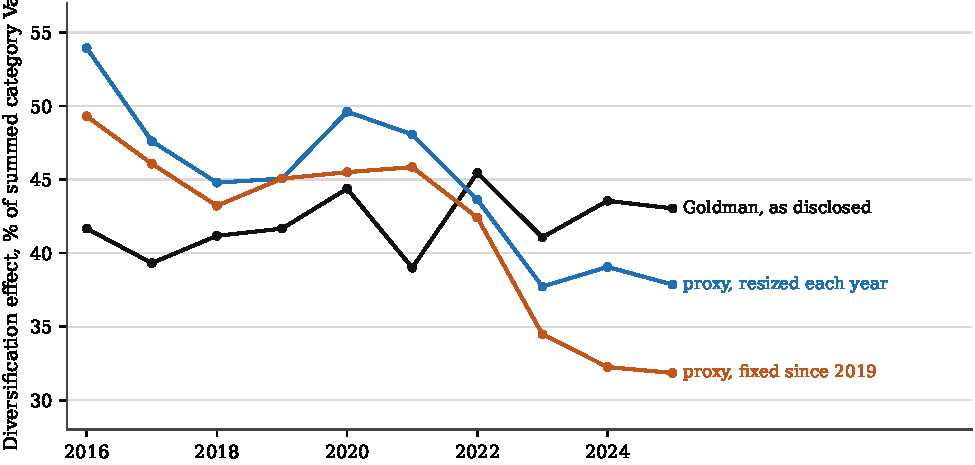
\includegraphics[width=\linewidth]{figures/diversification_over_time}
\caption{The disclosed diversification effect and the proxy book, FY2016--FY2025.
Goldman's series is flat across a decade containing a pandemic, a zero-rate
period and more than 500 basis points of policy tightening. Both proxy books
track it until 2022 and then decline, as the five-year scenario window fills
with the 2022 correlation regime and does not empty again.}
\label{fig:overtime}
\end{figure}

The mechanism is visible in the final column of Table~\ref{tab:results}. The
error in the fixed book's total VaR changes sign in 2022. Before then the proxy
over-diversifies, understating total VaR by as much as 21.0\%; afterwards it
under-diversifies, overstating total VaR by up to 9.1\%. The turn is the
equity--bond correlation moving positive in the inflation regime, which removes
the main diversifier available to a directional book. Goldman's ratio went
\emph{up} that year, to its sample maximum of 45.5\%.

The decline afterwards is a property of a long window on a static book. Once
2022 enters a five-year scenario set it stays there until 2027, so the measured
correlation structure keeps the inflation regime in view long after the market
has left it. Appendix~\ref{sec:appendix_c} cuts the same daily output into
market regimes, where the effect is starkest: the measured diversification
falls from 44.8\% in the calm years to 32.1\% in 2024--2025, on a book that
did not change. A dealer repositioning daily has no such ratchet, and
Section~\ref{sec:assumptions} shows that shortening or reweighting the window
does not rescue the result.

\subsection{Amplitude against persistence}

Goldman publishes the diversification effect twice: averaged over the year's
daily values, and as a period-end snapshot. Everything above compares the
average daily series, which is the measure the firm leads with. Comparing the
other one separates two things the first comparison conflates --- how far the
ratio moves, and whether those movements persist --- and the separation is
informative enough to change how the gap should be described.

% Generated by build/make_tables.py from gs_var_average_daily.csv, gs_var_period_end.csv and var_fixed_book_daily.csv. Do not edit.

\begin{table}[tbp]
\centering
\small
\caption{Amplitude and persistence: the two disclosed measures of the diversification effect against their proxy analogues}
\label{tab:amplitude}
\begin{tabular}{@{}lrrlrr@{}}
\toprule
 & & Std. & & Change, first & Lag-1 \\
Series & Mean & dev. & Range & half to second & autocorr. \\
\midrule
Goldman, average daily & 42.03 & 2.08 & 39.0--45.5 & +0.8 & -0.47 \\
Goldman, period-end & 38.21 & 6.72 & 28.6--48.6 & +8.6 & +0.07 \\
\addlinespace
Proxy, average daily & 41.60 & 6.33 & 31.9--49.3 & -8.5 & +0.88 \\
Proxy, final day of year & 40.62 & 6.68 & 30.6--47.8 & -10.2 & +0.90 \\
\bottomrule
\end{tabular}
\notetext{All figures are the diversification effect as a percentage of summed category VaR across the ten fiscal years, so each column rests on ten observations and none is precisely estimated. \emph{Change} is the mean of 2021--2025 less the mean of 2016--2020. \emph{Lag-1 autocorr.} is the correlation between consecutive annual values: negative indicates a series that returns toward its mean, positive one that carries its level forward. Neither disclosed series shows positive persistence --- the average daily series is $-0.47$ and the period-end series is essentially zero --- while both proxy series sit near $+0.9$. That contrast, rather than any difference in spread, is what Section~\ref{sec:results} rests on. No trend test is reported: the proxy's annual values are computed from overlapping five-year windows and share about 82\% of their scenario set with their neighbours, so a regression on them would understate its own standard errors.}
\end{table}


Table~\ref{tab:amplitude} sets both disclosed measures beside their proxy
analogues. The first thing it shows is that Goldman's ratio is not a stable
quantity. Measured period-end it has a standard deviation of 6.72 percentage
points and a range of 28.6 to 48.6, against 2.08 and 39.0 to 45.5 for the
average daily series. What is steady in the disclosures is the annual mean, not
the ratio.

The decisive column is the last one. The lag-1 autocorrelation of a series,
the correlation between consecutive annual values, distinguishes a quantity
that returns toward its mean from one that carries its level forward, and it
requires no model and no trend. Neither disclosed series shows positive
persistence: the average daily series is $-0.47$ and the period-end series is
essentially zero at $+0.07$. Both proxy series sit near $+0.9$. Whatever each
series does in a given year, Goldman's does not carry forward and the proxy's
does.

That is the finding, and it is sharper than a comparison of spreads. The proxy
does not fail to vary, nor vary too much; it fails to come back. Reading
Figure~\ref{fig:overtime} again with that in mind, the proxy lines do not
simply wobble more than the disclosed line; they leave and stay left.

The spread comparison corroborates this without carrying it. Measured
period-end against period-end the proxy's standard deviation is 6.68 against
Goldman's 6.72, which on inspection looks like an exact match and on
examination is not: each is estimated from ten observations, and the 95\%
confidence interval on the \emph{ratio} of the two runs from 0.50 to 2.02. The
defensible statement is that the two amplitudes are statistically
indistinguishable ($F = 1.01$, $p = 0.98$), which is weaker than reproduction
and is not evidence of equality. What the comparison does establish is that the
gap between the two average daily series is not simply a matter of the proxy
being more volatile, because measured alike the volatilities cannot be told
apart.

Two further qualifications. Each period-end figure is a single trading day, so
those rows rest on ten single-day observations and year-end snapshots may carry
balance-sheet effects an average does not. And the proxy's final trading day is
the last day of the aligned calendar rather than Goldman's fiscal period end.

\subsection{The configuration space}

A single calibration proves little, because the direction of each sleeve is not
disclosed and the diversification effect depends on those directions more than
on anything else in the specification. All sixteen sign combinations were
therefore run on the fixed book, and Figure~\ref{fig:frontier} plots each one's
decade-average level against its year-to-year standard deviation.

\begin{figure}[tbp]
\centering
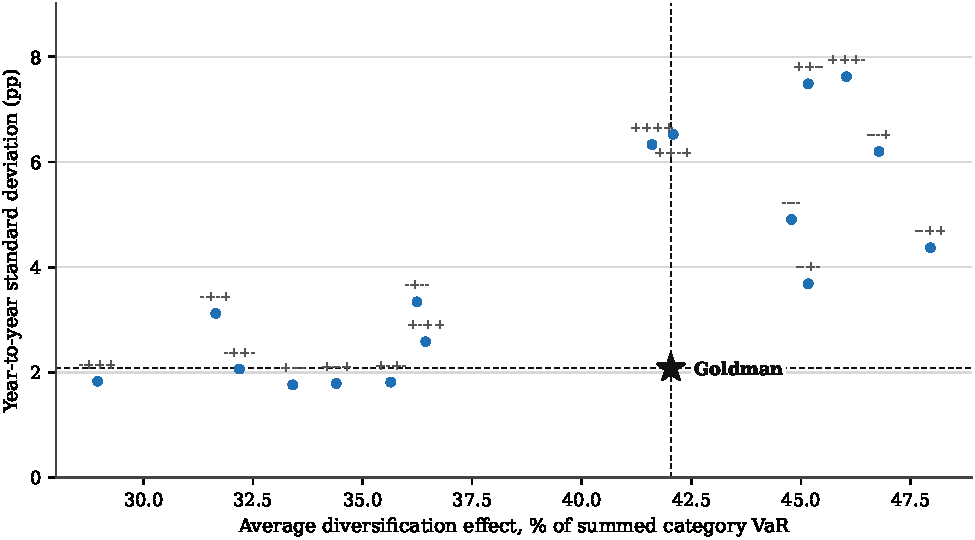
\includegraphics[width=\linewidth]{figures/stability_frontier}
\caption{Level against steadiness for all sixteen sleeve-sign configurations,
with Goldman's own position marked. Signs are in the order interest rates,
equity, currency, commodity. The dashed lines are Goldman's average level and
its year-to-year standard deviation; the quadrant below and to the right of
their intersection --- at least as steady as the disclosure, and at least as
high --- contains no configuration.}
\label{fig:frontier}
\end{figure}

Taking the disclosed standard deviation itself as the bar rather than a round
number chosen afterwards: five of the sixteen configurations are at least as
steady as Goldman's 2.08, and the highest of those averages 35.64\%, six points
below the disclosure. Eight average 40\% or more, and the steadiest of those
varies by 3.68 points a year, about 77\% more than Goldman. No configuration
achieves both.

This is a descriptive bound on what the engine can produce, and it should be
read as one rather than as a test. Every standard deviation in
Figure~\ref{fig:frontier} is estimated from ten annual observations and
carries a confidence interval spanning roughly a factor of two and a half in
each direction; the steadiest configuration's 3.68 and Goldman's 2.08 are not
separated by anything a formal comparison would certify. The sixteen
configurations are not independent draws either, since they share the same
factor data and differ only in sleeve signs, and the figures quoted are the
selected extremes across them, with no adjustment for that selection.

What the bound does establish is the shape of the trade-off. Within this
engine, moving a configuration toward Goldman's level moves it away from
Goldman's steadiness, across the whole sign space rather than at one point.
That is what makes the gap hard to explain away as a bad choice of signs: the
better choice would have to lie outside the space, and the space is complete.

\subsection{Backtest behaviour}

The engine's own coverage is reported here because it bears on how much weight
the diversification result can carry, and because it replicates a known finding
on a new sample. Table~\ref{tab:backtest} gives the four variants.

% Generated by build/make_tables.py from backtest_results.csv. Do not edit.

\begin{table}[tbp]
\centering
\footnotesize
\setlength{\tabcolsep}{4pt}
\caption{Backtest results on the fixed book}
\label{tab:backtest}
\begin{tabular}{@{}lllrrrrrrl@{}}
\toprule
Model & Conf. & Period & Days & Exc. & Rate (\%) & Kupiec & Indep. & Joint & Zone \\
\midrule
Historical simulation & 95\% & 2016-2025 & 2,293 & 160 & 6.98 & $<$0.0001 & $<$0.0001 & $<$0.0001 & red \\
Historical simulation & 95\% & 2020-2025 & 1,373 & 127 & 9.25 & $<$0.0001 & $<$0.0001 & $<$0.0001 & red \\
\addlinespace
Volatility weighted & 95\% & 2016-2025 & 2,293 & 117 & 5.10 & 0.822 & 0.110 & 0.272 & yellow \\
Volatility weighted & 95\% & 2020-2025 & 1,373 & 70 & 5.10 & 0.868 & 0.213 & 0.454 & yellow \\
\addlinespace
Historical simulation & 99\% & 2016-2025 & 2,293 & 45 & 1.96 & $<$0.0001 & $<$0.0001 & $<$0.0001 & red \\
Historical simulation & 99\% & 2020-2025 & 1,373 & 44 & 3.20 & $<$0.0001 & $<$0.0001 & $<$0.0001 & red \\
\addlinespace
Volatility weighted & 99\% & 2016-2025 & 2,293 & 19 & 0.83 & 0.395 & 0.573 & 0.594 & green \\
Volatility weighted & 99\% & 2020-2025 & 1,373 & 13 & 0.95 & 0.842 & 0.618 & 0.866 & green \\
\bottomrule
\end{tabular}
\notetext{Kupiec, Indep.\ and Joint are $p$-values for the proportion-of-failures, independence and conditional coverage tests. \emph{Zone} is the worst Basel traffic-light zone reached on any rolling 250-day window, computed at the confidence level of the row rather than at the published 99\% boundaries. The book is sized once on 2019, so the 2020--2025 rows are out of sample with respect to sizing.}
\end{table}


Plain historical simulation at the disclosed five-year window fails, and fails
on count as well as on arrangement: 160 exceptions in 2{,}293 days is a rate of
6.98\% against a nominal 5\%, which Kupiec rejects below any conventional
level, and the rate rises to 9.25\% from 2020. The failures cluster badly ---
70 of them fall in 2022 alone, out of 230 trading days --- and the model spends
18.2\% of days in the Basel red zone, peaking at 73 exceptions in a 250-day
window against a red threshold of 27.

Restating the scenario set in current volatility units repairs it. The
\citet{hullwhite1998} variant is not rejected by any of the three tests at
either confidence level: at 99\% it stays in the green zone throughout, peaking
at 4 exceptions in a 250-day window against a yellow threshold of 5. The
exception rate falls from 6.98\% to 5.10\% at 95\%, and the independence
statistic from 37.7 to 2.6.

This reproduces \citet{obrien2017evaluation} on a proxy book and a newer
sample. They found bank VaR exceedances excessive and clustered in the crisis,
and a conditional-volatility benchmark achieving lower exceedance rates without
clustering; the same pattern appears here, with the long disclosed window
standing in for the slow adjustment they document.

One comparison must be read carefully. Goldman disclosed 10 exceptions at 95\%
across the ten years, roughly 0.40\% of trading days against a nominal 5\%. A
literal coverage test on that count would reject calibration at any level, and
the rejection would be meaningless, because the two measurements are not the
same quantity. Goldman compares VaR against \emph{net revenues}, which include
intraday market-making income that is positive far more often than not; the
filings say so, and say it is why exceptions are rarer than the confidence
level implies. The proxy book has no client flow and no bid--offer spread, so
its profit and loss is a clean mark on a static position. The distance between
0.40\% and 5\% is an indication of how much the revenue cushion is worth, and
it is large, but it is not evidence that either model is miscalibrated. The
comparison is reported in Appendix~\ref{sec:appendix_a} and is not used
anywhere in this paper's conclusions.

% Drafted against audit/outline.md §7. Two deviations, both recorded in the
% outline: the sweeps table appears first (Table 8) and the candidate ledger
% second (Table 9), because the sweep is the evidence and the ledger is the
% summary; and the "tested at the disclosed settings, and refuted" subsection
% is new since the original outline, which predates the discovery that the
% disclosed window and weighting had never been implemented.
%
% Evidence: robustness_windows.csv, robustness_age_weighting.csv,
% robustness_sign_variants.csv, robustness_percentile.csv,
% convexity_comparison.csv, disclosed_var_commentary.csv, hash-recorded in
% audit/evidence_freeze.csv at commit 1e6bdd74.

\section{Which assumptions can explain the gap}\label{sec:assumptions}

Section~\ref{sec:results} established a gap: the disclosed diversification
effect moves by 2.08 percentage points a year and the proxy book's moves by
6.33. This section works through what could account for it, candidate by
candidate, and reports which survive.

\subsection{Ruled out by magnitude}

Two specification choices can be dismissed by size alone, without any argument
about mechanism.

The percentile convention is one. Reading the loss quantile by linear
interpolation rather than as a discrete order statistic moves average VaR by
0.30\% and the mean diversification ratio by 0.06 percentage points. Convexity
is the other. Pricing the rate sleeve by full revaluation rather than by a
duration approximation moves annual average VaR by between 0.25\% and 0.59\%,
with a largest single-day gap of 1.55\%. Neither is within two orders of
magnitude of a four-point discrepancy in a ratio's standard deviation.

Both are worth running anyway, because an unexamined choice is an unexamined
choice, and because the convexity comparison establishes something useful in
its own right: on a one-day horizon with daily yield moves of about five basis
points, full revaluation on vanilla bonds buys three tenths of a percent. It
earns its cost on instruments whose value is sharply non-linear in the factor,
which means options, and on longer horizons. That is a finding about method
rather than about Goldman.

\subsection{Right direction, not far enough}

The scenario window is a real effect and the first candidate that moves the
result.

The top block of Table~\ref{tab:sweeps} runs the window at one, two, three and
five years with equal weights. Steadiness improves monotonically as the window
lengthens: the year-to-year standard deviation falls from 10.23 points at one
year to 8.87 at two, 8.36 at three and 6.33 at the disclosed five. The level
climbs toward the disclosure at the same time, from 38.2\% to 41.6\% against
42.0\%.

% Generated by build/make_tables.py from robustness_windows.csv and robustness_age_weighting.csv. Do not edit.

\begin{table}[tbp]
\centering
\small
\caption{Steadiness and coverage move in opposite directions under Goldman's own disclosed settings}
\label{tab:sweeps}
\begin{tabular}{@{}llrrrr@{}}
\toprule
 & Half-life & Mean & Year-to-year & Exception & \\
Specification & (days) & (\%) & std.\ dev.\ (pp) & rate (\%) & Kupiec \\
\midrule
\multicolumn{6}{@{}l}{\emph{Lookback window, equally weighted}} \\
252 days (1y) & --- & 38.2 & 10.23 & 5.58 & 0.209 \\
502 days (2y) & --- & 39.0 & 8.87 & 5.58 & 0.209 \\
756 days (3y) & --- & 39.6 & 8.36 & 5.89 & 0.058 \\
1,260 days (5y)\;$\dagger$ & --- & 41.6 & 6.33 & 6.98 & $<$0.0001 \\
\addlinespace
\multicolumn{6}{@{}l}{\emph{Scenario age weighting, at the disclosed window}} \\
$\lambda = 1.00$ (equal) & --- & 41.6 & 6.33 & 6.98 & $<$0.0001 \\
$\lambda = 0.99$ & 69 & 39.9 & 10.04 & 5.45 & 0.328 \\
$\lambda = 0.97$ & 23 & 42.0 & 9.46 & 5.63 & 0.177 \\
\midrule
\emph{Goldman, as disclosed} & --- & 42.0 & 2.08 & 0.40 & --- \\
\bottomrule
\end{tabular}
\notetext{$\dagger$ marks the disclosed window. The top block holds the weighting equal and varies the window length; the lower block holds the window at the disclosed five years and varies the decay. Reading down the lower block, the year-to-year standard deviation rises while the exception rate falls toward its nominal 5\% and Kupiec stops rejecting: adopting Goldman's disclosed weighting makes the engine a better risk model and a worse reproduction of the disclosed steadiness, at the same time. Goldman's own exception rate is measured against net revenues and is not comparable; it is shown for scale only and discussed in Section~\ref{sec:results}.}
\end{table}


The direction is right and the destination is not. Five years is the end of
this road rather than a point along it, because five years is what Goldman
discloses: there is no longer window to appeal to. At the disclosed length
the ratio still moves three times as much as the disclosed series, and the
engine's coverage has deteriorated badly in the process: the exception rate
rises from 5.58\% at one year to 6.98\% at five, and Kupiec goes from not
rejecting to rejecting below any conventional level. A five-year equally
weighted scenario set is slow, and 2022 is where that shows: 70 exceptions in
230 trading days, because five years of scenarios in early 2022 reached back
to 2017 and contained almost no rate volatility.

\subsection{Tested at the disclosed settings, and refuted}

The obvious objection to everything above is that a seventeen-factor proxy is a
blunter instrument than Goldman's, so the gap measures the replication rather
than the bank. The disclosed age weighting tests that objection directly,
because it is the one remaining piece of Goldman's stated method that had not
been applied, and because it bears on exactly the quantity in dispute: how
quickly the engine's view of the correlation structure turns over.

It does not close the gap. It widens it. The lower block of
Table~\ref{tab:sweeps} holds the window at the disclosed five years and varies
the decay. At a 69-day half-life the year-to-year standard deviation rises from
6.33 to 10.04 points; at a 23-day half-life, to 9.46. Against a disclosed 2.08,
adopting Goldman's own weighting takes the engine from three times too variable
to four or five times too variable.

And it does so while making the engine a better risk model by every coverage
test applied to it. The exception rate falls from 6.98\% to 5.45\% at the
longer half-life and 5.63\% at the shorter, both close to the nominal 5\%.
Kupiec's $p$-value rises from below 0.0001 to 0.328 and 0.177 respectively, and
at the faster decay the independence test passes as well, at 0.305. Weighting
toward recent observations is the correct specification for a
historical-simulation engine; the filings say so in plain terms, and the
backtest agrees with them.

The two movements are in opposite directions and that is the point. Reading
down the lower block of Table~\ref{tab:sweeps}, coverage improves and
steadiness degrades together. The gap between the disclosed steadiness and the
reproduced steadiness is therefore not an artefact of this replication using a
cruder method than the bank. It uses the bank's method, the bank's own window
and weighting scheme, and the gap gets larger.

The filings disclose the weighting in kind but not in degree: they say the
importance of the data reduces over time without giving the rate. Two rates
cannot establish what every rate would do, so the parameter was swept across
sixteen values spanning half-lives from 6.6 trading days to 1{,}386, and
Figure~\ref{fig:decay} reports the result.

The relationship is not monotone, which is worth saying plainly because the
obvious argument, that faster decay turns the scenario set over faster and
so must increase variability, is wrong. Year-to-year variability rises
steeply as decay is introduced, peaks at 10.04 points around a 69-day
half-life, and then falls back to 8.65 at the fastest rate tested. The
conclusion survives the correction and is now demonstrated rather than
asserted: the steadiest configuration anywhere in the grid is equal weighting
itself, at 6.33, and every weighted configuration is further from the
disclosures than that. The minimum across all sixteen rates is three times
Goldman's 2.08.

\begin{figure}[tbp]
\centering
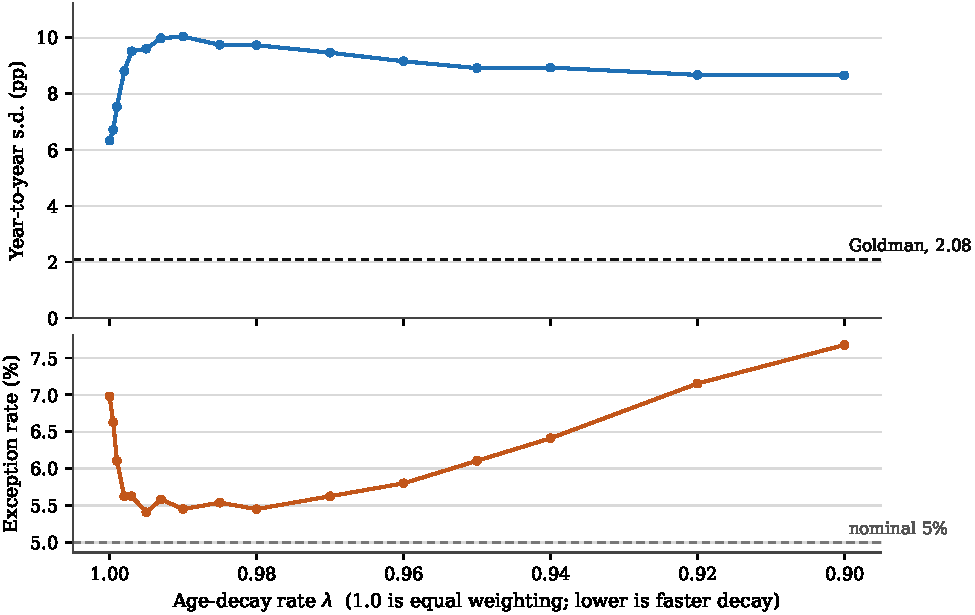
\includegraphics[width=\linewidth]{figures/decay_grid}
\caption{Year-to-year variability and coverage against the age-decay rate, at
the disclosed five-year window. Sixteen rates, from equal weighting to a
6.6-day half-life. The upper panel never approaches Goldman's 2.08 anywhere in
the grid, and its minimum is equal weighting. The lower panel reaches the
nominal 5\% exception rate in the middle of the range, where the upper panel
is near its worst.}
\label{fig:decay}
\end{figure}

The lower panel shows the opposing movement across the whole grid rather than
at two points. Coverage is best near a 138-day half-life, where the exception
rate is 5.41\% against a nominal 5\% and Kupiec's $p$-value reaches 0.376,
and the year-to-year variability there is 9.61, among the worst in the sweep.
There is no rate at which the engine is both well calibrated and as steady as
the disclosures, and the sweep is dense enough to say so.

\subsection{Bounded by the configuration space}

Sleeve direction remains the specification choice with the largest effect on
the diversification effect, and Section~\ref{sec:results} reported the bound:
across all sixteen sign configurations, five are at least as steady as the
disclosure and the best of those averages 35.6\%, while eight reach 40\% or
more and the steadiest of those varies by 3.68 points. None does both.

What that bound rules out is a particular kind of objection: that the long-only
baseline is simply the wrong corner of the space, and some other corner would
land on Goldman. It would have to be a corner that is not in the space. The
sixteen configurations exhaust the sign choices available to a four-sleeve
book, and the empty quadrant in Figure~\ref{fig:frontier} is a property of all
of them.

\subsection{What survives}

Three candidates the frozen evidence cannot exclude, and they are not ranked,
because nothing here ranks them.

\emph{The factor count.} Seventeen factors against the roughly 70,000 the
FY2016 and FY2017 filings describe. More independent sources of risk means more
diversification available, so the direction of the bias on the \emph{level} is
known. The direction on the \emph{steadiness} is not: a larger factor set might
average out regime shifts in any one correlation, or might not. Nothing in
public data settles it, and this paper does not guess.

\emph{Non-synchronous closes.} Tokyo, London and New York do not close at the
same instant, which depresses measured cross-market correlation and therefore
overstates diversification. This runs opposite to the factor-count bias, which
is why neither is used to argue the result in either direction. Neither is
quantified.

Table~\ref{tab:candidates} summarises the three verdicts below alongside the
exclusions above.

\emph{Exposure management.} This is the candidate with direct evidence behind
it, and Section~\ref{sec:results} sharpened what it has to explain. A static
book cannot reproduce a path produced by a desk that trades against the market,
and Goldman's own commentary says that is what the desk does. In four
consecutive filings --- FY2021 through FY2024 --- the explanation of the
year-over-year VaR change has the same shape: volatility moved one way,
``partially offset by'' exposures moving the other. The firm also moved
positions in and out of the measure outright, as the first-quarter 2023 scope
change shows. A book whose notionals were fixed in 2019 has no counterpart to
any of that.

What Table~\ref{tab:amplitude} adds is that this candidate now has a specific
job. It does not need to explain why Goldman's ratio moves less than the
proxy's, because on a like-for-like basis it does not: period-end against
period-end the two have almost the same year-to-year variation. It needs to
explain why Goldman's movements revert and the proxy's accumulate. Exposure
management is a mechanism that would do exactly that. A desk that sells risk
into a correlation regime it dislikes and buys it back when the regime passes
produces a ratio that wanders and returns; a fixed book exposed to the same
market produces one that wanders and stays. Nothing in the public data
establishes that this is what happens, but of the three surviving candidates it
is the only one whose mechanism matches the shape of the discrepancy.

% Generated by build/make_tables.py from the robustness and comparison outputs. Do not edit.

\begin{table}[tbp]
\centering
\footnotesize
\setlength{\tabcolsep}{5pt}
\caption{Candidate explanations for the steadiness gap, and what settles each}
\label{tab:candidates}
\begin{tabularx}{\linewidth}{@{}l Y l@{}}
\toprule
Candidate & What settles it & Verdict \\
\midrule
Percentile convention & Moves VaR by 0.30\% and the mean ratio by 0.06 pp & Excluded \\
Convexity in the rate sleeve & Full revaluation against duration moves annual VaR by at most 0.59\% & Excluded \\
Lookback window too short & Lengthening 1y$\rightarrow$5y cuts the gap from 10.23 to 6.33 pp, against 2.08 & Right way, insufficient \\
Equal weighting, not Goldman's & Swept over 16 decay rates: the steadiest is equal weighting at 6.33 pp and every weighted rate is worse, while coverage improves & Refuted \\
Wrong sleeve directions & Of 16 configurations, 5 match the steadiness and peak at 35.6\%; 8 match the level and bottom out at 3.68 pp & Excluded \\
Seventeen factors, not 70{,}000 & Not testable on public data; biases the level downward, direction on steadiness unknown & Survives \\
Non-synchronous closes & Depresses measured cross-market correlation; magnitude not estimated & Survives \\
Exposures are managed, not held & Goldman attributes VaR changes to exposure moves in four consecutive filings; the only candidate whose mechanism produces reversion rather than drift & Survives \\
\bottomrule
\end{tabularx}
\notetext{The disclosed year-to-year standard deviation is 2.08 percentage points; every quantity in the middle column is measured against that. \emph{Refuted} is stronger than \emph{excluded}: the disclosed weighting was adopted and moved the gap the wrong way. The three surviving candidates are not ranked, because nothing in the frozen evidence ranks them.}
\end{table}


\subsection{Taken together}

The gap survives the removal of every specification choice that could be
removed. It is not the percentile rule, not convexity, not the window length,
not the weighting scheme, and not the sleeve signs. What remains is structural:
a static four-sleeve book exposed to seventeen public factors, against a
trading operation with a far larger factor set that repositions daily.

It is worth restating what the gap is, now that Section~\ref{sec:results} has
narrowed it. The proxy is not insufficiently variable or excessively variable
relative to the disclosures; measured on the same basis its variation is almost
identical in size. The proxy's variation persists where Goldman's reverts, and
every candidate above has been tested against that discrepancy rather than
against a difference in amplitude that does not exist.

\citet{danielsson2016modelrisk} give the mechanism in general form. Model risk,
the tendency of different models to disagree, rises with market
uncertainty: candidate models agree in calm periods and diverge significantly
in distress. Read through the diversification ratio, that is what
Section~\ref{sec:results} reports. The proxy tracks the disclosure closely
through the calm years to 2021, and separates from it in 2022 and after.
Their object is risk forecasts in general rather than a disclosed
diversification effect, so this is an application of their finding rather than
a confirmation of it.

The reading this paper settles on is narrow by design. A static book cannot
hold a diversification ratio near 42\% through both 2021 and 2023, because the
correlation structure beneath it changed and the book did not. Goldman's did
hold. Whatever accounts for that is not in the methodology the filings
disclose, because the methodology the filings disclose has been applied here
and does not produce it.

% Drafted against audit/outline.md §8. Two additions to the outline's five
% bullets, both of which became limitations only after the disclosed-settings
% rerun: the undisclosed decay rate, and the fact that the disclosed window
% leaves no room to appeal to a longer one. Recorded in the outline.
%
% No new evidence. Everything here is carried from §3, §4 and §7.

\section{Limitations}\label{sec:limitations}

Everything in this section constrains how the results should be read. The two
that matter most run in opposite directions, and the paper does not claim they
cancel.

\subsection{Seventeen factors against roughly seventy thousand}

This is the largest single difference between the engine here and Goldman's,
and it is not fixable from public data. More independent sources of risk means
more offsetting available in the joint tail, so a seventeen-factor book should
show \emph{less} diversification than a book with a richer factor set. The
direction of that bias on the level is therefore known, and it makes the level
agreement in Section~\ref{sec:results} slightly surprising rather than
suspicious.

The direction on the steadiness is not known, and that is the more important
gap. A larger factor set might average out regime shifts in any one
correlation, which would push toward the disclosed stability; or it might not,
if the shifts are common across factors, which is what a macro regime change
usually means. Nothing in public data settles it. Section~\ref{sec:assumptions}
lists it as a surviving candidate and declines to guess, and the central result
should be read with that candidate open.

\subsection{Non-synchronous closes}

Tokyo, London and New York do not close at the same instant. A move that
happens in New York after the Tokyo close appears in the Japanese series only
the following day, which mechanically depresses measured cross-market
correlation and therefore \emph{overstates} diversification.

This runs opposite to the factor-count bias. Neither is quantified here, and
the two are not assumed to offset: they are stated so that a reader knows the
measured level sits between two unestimated biases of unknown relative size.
This is also why neither is used anywhere to argue that the result would move
in a particular direction if corrected.

\subsection{What the calendar intersection costs}

Restricting the panel to days on which every market traded discards about 9\%
of trading days and leaves 225 to 233 observations a year against the 250 to
253 Goldman reports. The alternative --- forward-filling closed markets ---
would plant runs of exact zeros in the scenario set and understate those
factors' risk, which biases the quantity being measured rather than merely
reducing the precision of the measurement. The smaller sample is the better of
two imperfect options, but it does cost power in every test in
Section~\ref{sec:validation}, and the annual figures rest on fewer observations
than the disclosures they are compared against.

A related quantisation affects the rate factors. The Treasury curve is quoted
to the basis point, so at near-zero policy rates the two-year yield shows no
change at all on 21.1\% of days across the panel and 43.1\% of days in the
second half of 2020. That is a real feature of the quoted series rather than a
data error, and it slightly understates true rate variability through the
near-zero years.

\subsection{Instrument substitutions}

Commodity exposure runs through exchange-traded funds rather than front-month
futures, for the reason given in Section~\ref{sec:sample}. Funds carry roll
yield, which drags them away from spot over long horizons. Over the one-day
horizon the engine uses it is second order, but it is a real difference from a
spot book and it is not corrected.

The rate sleeve mixes US par coupon bonds with euro zero-coupon bonds, each in
its source curve's native convention. A zero has longer duration than a par
bond of the same maturity, so the two are not interchangeable per unit of
notional. Sizing targets risk rather than notional, which absorbs the
difference for the purpose of matching the disclosed split, but the instrument
sets are not identical and a reader comparing notionals across sleeves in
Table~\ref{tab:book} should not read them as comparable exposures.

\subsection{What the recalibrated book cannot be used for}

The recalibrated book is sized each year using figures Goldman published after
that year ended: the 2022 sizing uses a figure released in February 2023. That
is appropriate for the structural comparison it is used for, because the
question is whether a book with the disclosed risk split generates the
disclosed co-movement, and the split is the input. It would be indefensible as
a forecast. This is why only the fixed book, sized once on 2019 and never
touched again, is backtested, and why the 2020--2025 rows of
Table~\ref{tab:backtest} are out of sample with respect to sizing.

\subsection{Two limits the disclosed settings impose}

Adopting Goldman's stated method closed some latitude and opened a different
constraint.

The decay rate behind the disclosed age weighting is not published. The filings
say the importance of the data reduces over time without saying how fast, so
the scheme is tested in kind but not at Goldman's own rate. The two rates run
here were chosen for their half-lives and both move the steadiness the same
way, which is what makes the conclusion in Section~\ref{sec:assumptions} robust
to not knowing the rate, but it remains a conclusion about a family of decay
rates rather than about Goldman's.

The window leaves no further room. Five years is what the filings disclose, so
the monotone improvement in steadiness with window length cannot be extended by
appeal to a longer one. That is a limitation on the argument's escape routes
rather than on its evidence: the result is bounded by what the firm says it
does.

\subsection{What validation does not cover}

Finally, and most importantly for interpretation: Section~\ref{sec:validation}
establishes that the engine computes what Section~\ref{sec:method} says it
computes. It does not establish --- and no test on public data could --- that
the proxy book resembles Goldman's trading book. The level agreement is
evidence about the proxy, and the steadiness gap is evidence about what a
static proxy cannot do. Neither is a measurement of anything inside the firm.

% Drafted against audit/outline.md §9. No new evidence and no new citations.
% Every figure restated here appears with its verification in §6 or §7.

\section{Conclusion}\label{sec:conclusion}

Goldman Sachs discloses one number in Item 7A that depends on something the
filing never publishes. The four category VaRs are levels; the diversification
effect is a relationship, and it is the only line in the table that a reader
outside the firm can test without knowing a single position. This paper tested
it, over ten consecutive fiscal years, with a historical-simulation engine run
at the bank's own disclosed settings on seventeen public risk factors.

The level transfers. A book sized once on 2019 and then left alone averages
41.6\% of summed category VaR against a disclosed 42.0\%, a difference no test
on ten annual observations distinguishes from zero. That corroborates
\citet{perignon2010diversification}, who found disclosed diversification
effects close to independently estimated ones on four US banks and quarterly
data ending in early 2007. Finding it again on a different bank, a different
decade, a different frequency and a different method is worth reporting
precisely because it is not new: a result that survives that much substitution
is a result about disclosure practice rather than about one estimation.

The steadiness does not transfer, and that is what this paper adds. Goldman's
average daily ratio has a year-to-year standard deviation of 2.08 percentage
points across a decade containing a pandemic, a zero-rate period and more than
500 basis points of policy tightening. The proxy's is 6.33, a difference a
variance-ratio test puts at $p = 0.0028$, and the two move oppositely over the
sample: Goldman's second-half mean is 0.8 points above its first, the proxy's
8.5 below.

The firm's second disclosed measure says what kind of failure it is. Goldman
also publishes a period-end snapshot of the same ratio, and that series has a
standard deviation of 6.72 points. Its diversification effect moves a great
deal, and what is stable is the annual mean rather than the quantity. Measured
period-end against period-end, the proxy's variation cannot be distinguished
from Goldman's. What distinguishes them is persistence: the lag-1
autocorrelation of consecutive annual values is $-0.47$ for Goldman's average
daily series and about zero for its period-end series, against roughly $+0.9$
for both proxy series. Goldman's movements do not carry forward; the proxy's
do. The proxy reproduces the level, and its variation is the same size as the
disclosed variation; what it fails to reproduce is the mean reversion, and the
mean reversion is what the disclosed steadiness consists of.

What makes the result hard to dismiss is that it survives being handed the
bank's own method. The filings disclose a five-year scenario window and
age-weighted scenarios, and both were implemented. The window moves the gap the
right way and runs out of room, since five years is what is disclosed and there
is no longer window to appeal to, and the weighting moves it the wrong way,
raising the standard deviation to between 9.46 and 10.04 points while
simultaneously repairing the engine's coverage, from a 6.98\% exception rate
that Kupiec rejects below 0.0001 to 5.45\% at $p = 0.328$. The engine gets
better as a risk model and worse as a reproduction of the disclosed steadiness,
in the same move. Whatever holds Goldman's ratio still is not in the
methodology the filings describe, because that methodology has been applied
here and does not produce it.

Nor is it a matter of having guessed the sleeve directions wrongly. Across all
sixteen sign configurations the two properties trade off: five are at least as
steady as the disclosure and the best of those averages 35.6\%, eight reach
40\% or more and the steadiest of those varies by 3.68 points. None does both.
That trade-off, rather than any single calibration, is what the sign space
establishes. It is a descriptive bound on what this engine can produce rather
than a test --- ten annual observations per configuration will not support one
--- and it is what an outside party can establish from public data.

Taken with the decomposition above, the paper's contribution is two-part: a
replication run at the bank's own disclosed settings, which rules out the
objection that the gap measures a cruder method; and a separation of amplitude
from persistence using a second disclosed series the firm already publishes,
which identifies what the gap actually consists of. Neither requires anything
the filings do not contain.

\subsection*{How much this establishes, and how much it does not}

The claim is narrower than the result might be made to sound. This paper does
not show that Goldman's disclosed diversification effect is implausible,
managed, or anything other than what the firm says it is. It shows that a
static four-sleeve book of public factors cannot reproduce it, under the
method the firm discloses, across the full space of sign configurations
available to such a book. Those are different statements, and the second does
not imply the first.

Three explanations survive the elimination in Section~\ref{sec:assumptions},
and the paper does not rank them because nothing in the evidence ranks them.
The factor count, seventeen against roughly seventy thousand, is the
largest structural difference and its effect on steadiness is simply unknown.
Non-synchronous closes across time zones bias the measurement in the opposite
direction to the factor count, and neither bias is quantified. And exposures
are managed rather than held: in four consecutive filings, FY2021 through
FY2024, Goldman attributes its year-over-year VaR change to volatility moving
one way and exposures moving the other. A book whose notionals were fixed in
2019 has no counterpart to that. It is the one surviving candidate with direct
documentary support, and the only one whose mechanism matches the shape of the
discrepancy: a desk that sheds risk into an unwelcome correlation regime and
restores it afterwards produces a ratio that returns to where it was, which is
precisely what the proxy's does not do.

\subsection*{What would settle it}

Separating those three requires data that is not public. Position-level or
desk-level exposures would do it directly: holding the factor set fixed and
varying only whether positions are repriced or held would isolate exposure
management from the other two, and a richer factor set run against the same
book would isolate the factor count. Supervisory data of the kind
\citet{obrien2017evaluation} worked with would get part of the way, though it
carries the trading outcomes rather than the diversification decomposition this
question needs.

Absent any of that, the bound is what an outside party can establish, and
establishing it is the point. A reader of a 10-K can now say something specific
about the one line in the market-risk table that is testable from outside: its
level is reproducible from public data, the size of its variation is
reproducible too, and its persistence is not, under the bank's own disclosed
window and weighting, swept across the range the filings leave open.

% Unnumbered back matter, in the same set and the same order as the author's
% previous working paper: Funding, Disclosure statement, Data availability
% statement, Code availability, Declaration of generative AI use.
%
% The availability statements are written for this project rather than carried
% over, which is what the previous paper did relative to its own predecessor:
% the inputs here are ten SEC filings and three public market-data endpoints,
% not pricing supplements and option chains, so copying that text would
% describe a study that does not exist.
%
% The generative-AI-use declaration keeps the earlier paper's wording and
% position. As in that paper, this section is a documented exception to the
% repository's vocabulary check and should be listed as such wherever that
% check is run.

\section*{Funding}
The author declares no external funding.

\section*{Disclosure statement}
The author declares no competing financial interests. The author holds no
position in, and has no commercial relationship with, The Goldman Sachs Group,
Inc.

\section*{Data availability statement}
Every input to this study is public. The ten Form 10-K filings are listed with
their accession numbers in Table~\ref{tab:manifest} and remain retrievable from
EDGAR; the Market Risk Management section of each is preserved verbatim under
\texttt{references/sec\_filings/}, which is the text every disclosed figure was
read from, and the parsed series are tracked as CSV so the disclosed side of
every comparison can be inspected without running anything.

The market data behind the factor panel cannot be preserved the same way. The
US Treasury par yield curve is a work of the US government and the European
Central Bank's euro area curve is openly licensed with attribution; either
could be redistributed. The exchange-traded closes come from a commercial
endpoint whose terms do not permit redistribution, and because the aligned
panel interleaves all three sources, no part of it is tracked. What is tracked
is \texttt{scripts/02\_build\_factors.py}, which rebuilds the panel from the
same public endpoints over the window recorded in \texttt{config/params.yaml}.
A reader reproducing this paper regenerates the factor data rather than
receiving it.

\section*{Code availability}
The disclosure retrieval and parser, the factor construction, the
Value-at-Risk engine, the calibration, the backtest, the regime and robustness
analyses and the test suite described in Section~\ref{sec:validation} are all
available in the repository. Every table and figure in this paper is generated
from the tracked analysis outputs by a script under the manuscript's own
\texttt{build/} directory; none is transcribed by hand, and deleting the
generated files and rerunning those scripts reproduces the manuscript
unchanged. One exception is worth naming: Table~\ref{tab:factorstats} reads
the aligned factor panel for the sentence recording how many trading days it
spans, and that panel is the one input not tracked, for the reason given
above. Rebuilding it restores the table; skipping it costs that table and
nothing else. The commit the reported results were produced from, together with a
SHA-256 digest of each analysis output they depend on, is recorded under
\texttt{audit/}, so a reader can confirm that a given number corresponds to the
state of the code that produced it.

\section*{Declaration of generative AI use}
During the preparation of this work, the author used Claude in order to revise
and restructure the manuscript, prepare the plotting script, literature checks
and LaTeX preparation. After using this tool/service, the author reviewed and
edited the content as needed and takes full responsibility for the content of
the published article.


\begingroup
\small
\setlength{\bibsep}{4pt}
\bibliographystyle{apacite}
\bibliography{references/references}
\endgroup

\appendix
% \appendix letters the sections but leaves floats on the main sequence, so an
% appendix table would arrive as "Table 11" with no hint of where it lives.
% counterwithin both prefixes the letter and resets the count per appendix,
% which a bare \setcounter does only once.
\counterwithin{table}{section}
\counterwithin{figure}{section}
% Appendix A. The disclosed series in full, plus the exception comparison
% that §6 defers here. Tables generated by build/make_tables.py.

\section{The disclosed series in full}\label{sec:appendix_a}

Table~\ref{tab:manifest} identifies the ten filings every disclosed figure in
this paper is read from. Accession numbers are given so that any figure can be
traced to the document it came from and retrieved independently.

% Generated by build/make_tables.py from gs_filing_manifest.csv. Do not edit.

\begin{table}[tbp]
\centering
\small
\caption{The filings the disclosed series is read from}
\label{tab:manifest}
\begin{tabular}{@{}llll@{}}
\toprule
Fiscal year & Period end & Filed & Accession number \\
\midrule
FY2016 & 2016-12-31 & 2017-02-27 & \texttt{0001193125-17-056804} \\
FY2017 & 2017-12-31 & 2018-02-26 & \texttt{0001193125-18-056383} \\
FY2018 & 2018-12-31 & 2019-02-26 & \texttt{0001193125-19-050198} \\
FY2019 & 2019-12-31 & 2020-02-21 & \texttt{0001193125-20-043853} \\
FY2020 & 2020-12-31 & 2021-02-22 & \texttt{0001193125-21-049380} \\
FY2021 & 2021-12-31 & 2022-02-25 & \texttt{0001193125-22-052682} \\
FY2022 & 2022-12-31 & 2023-02-24 & \texttt{0000886982-23-000003} \\
FY2023 & 2023-12-31 & 2024-02-23 & \texttt{0000886982-24-000006} \\
FY2024 & 2024-12-31 & 2025-02-27 & \texttt{0000886982-25-000005} \\
FY2025 & 2025-12-31 & 2026-02-25 & \texttt{0000886982-26-000091} \\
\bottomrule
\end{tabular}
\notetext{The Goldman Sachs Group, Inc., Annual Report on Form 10-K, CIK 0000886982. Each is retrievable from EDGAR at \path{https://www.sec.gov/Archives/edgar/data/886982/<accession>/}. Every figure in this paper is taken from the Market Risk Management section of one of these ten documents.}
\end{table}


Table~\ref{tab:disclosed} in Section~\ref{sec:disclosed} gives the average
daily series, which is what the analysis uses. Table~\ref{tab:periodend} gives
the period-end series for completeness. The two measure different things: the
average daily figure summarises a year of risk-taking, while the period-end
figure is a single day's snapshot and is correspondingly noisier. The
diversification identity holds in both.

% Generated by build/make_tables.py from gs_var_period_end.csv. Do not edit.

\begin{table}[tbp]
\centering
\small
\caption{Period-end Value-at-Risk by risk category, FY2016--FY2025}
\label{tab:periodend}
\begin{tabular}{@{}lrrrrrrrr@{}}
\toprule
 & \multicolumn{4}{c}{Risk category} & & & & \\
\cmidrule(lr){2-5}
Year & Rates & Equities & FX & Commod. & Summed & Diversif. & Total & \% of sum \\
\midrule
2016 & 45 & 34 & 23 & 19 & 121 & -39 & 82 & 32.2 \\
2017 & 48 & 31 & 7 & 9 & 95 & -30 & 65 & 31.6 \\
2018 & 46 & 32 & 12 & 11 & 101 & -44 & 57 & 43.6 \\
2019 & 54 & 24 & 10 & 10 & 98 & -28 & 70 & 28.6 \\
2020 & 60 & 50 & 11 & 16 & 137 & -46 & 91 & 33.6 \\
2021 & 69 & 31 & 19 & 30 & 149 & -58 & 91 & 38.9 \\
2022 & 108 & 27 & 35 & 18 & 188 & -85 & 103 & 45.2 \\
2023 & 93 & 25 & 15 & 14 & 147 & -54 & 93 & 36.7 \\
2024 & 84 & 41 & 38 & 14 & 177 & -86 & 91 & 48.6 \\
2025 & 59 & 45 & 17 & 18 & 139 & -60 & 79 & 43.2 \\
\bottomrule
\end{tabular}
\notetext{In millions of US dollars, except the final column. The analysis in this paper uses average daily VaR (Table~\ref{tab:disclosed}); the period-end series is a single-day snapshot and is reported here for completeness. The identity holds in this series too.}
\end{table}


Section~\ref{sec:results} uses the period-end series to separate the amplitude
of the disclosed variation from its persistence, and Table~\ref{tab:amplitude}
carries that comparison. The point in brief: measured period-end Goldman's own
ratio has a year-to-year standard deviation of 6.72 percentage points against
2.08 for the average daily series, so the disclosed steadiness is a property of
the annual mean rather than of the ratio itself.

The disclosed high and low VaR by category point the same way. Taken as first
reported, the median within-year ratio of high to low runs from 1.9 for
interest rates to 4.3 for currency rates. A book whose category VaRs move
through ranges that wide over a year is not a book whose diversification effect
sits still from day to day, and the filings are explicit enough about this that
no inference is needed.

\subsection*{Exception counts}

Section~\ref{sec:results} defers this comparison here because it cannot carry
weight. Table~\ref{tab:exceptions} gives it.

% Generated by build/make_tables.py from exceptions_vs_disclosed.csv. Do not edit.

\begin{table}[tbp]
\centering
\small
\caption{Exception counts at 95\%: the proxy book against Goldman's disclosed counts}
\label{tab:exceptions}
\begin{tabular}{@{}lrrrr@{}}
\toprule
 & \multicolumn{3}{c}{Proxy book, plain historical simulation} & Goldman \\
\cmidrule(lr){2-4}
Year & Days & Exceptions & Rate (\%) & Exceptions \\
\midrule
2016 & 233 & 9 & 3.9 & 0 \\
2017 & 232 & 5 & 2.2 & 0 \\
2018 & 230 & 11 & 4.8 & 2 \\
2019 & 225 & 8 & 3.6 & 0 \\
2020 & 227 & 12 & 5.3 & 2 \\
2021 & 231 & 11 & 4.8 & 1 \\
2022 & 230 & 70 & 30.4 & 2 \\
2023 & 233 & 19 & 8.2 & 1 \\
2024 & 228 & 11 & 4.8 & 2 \\
2025 & 224 & 4 & 1.8 & 0 \\
\midrule
Total & 2,293 & 160 & 6.98 & 10 \\
\bottomrule
\end{tabular}
\notetext{\textbf{These two columns do not measure the same thing and should not be compared as though they did.} Goldman scores VaR against daily net revenues, which include intraday market-making income that is positive far more often than not; the proxy book has no client flow and no bid--offer spread, so its profit and loss is a clean mark on a static position. The table is reported for completeness and the gap is an indication of what the revenue cushion is worth, not evidence that either model is miscalibrated. No conclusion in this paper rests on it.}
\end{table}


Goldman recorded 10 exceptions at the 95\% risk-management measure across the
ten years, against 160 for the proxy book. The gap is not evidence about either
model's calibration, because the two are scored against different quantities:
Goldman compares VaR against daily net revenues, which include intraday
market-making income that is positive on the large majority of days, while the
proxy book is a static position marked cleanly with no client flow and no
bid--offer spread. The filings make this point themselves, observing that in
periods with far more positive than negative net revenue days, fewer exceptions
are expected than the confidence level implies.

The distance between 0.40\% and 6.98\% of days is therefore best read as an
indication of how much the revenue cushion is worth, and it is large. It is not
used anywhere in this paper's conclusions.

% Appendix B. Implementation detail that would interrupt §4 but that a
% reader reimplementing the engine needs. No floats.

\section{Engine specification}\label{sec:appendix_b}

This appendix records three implementation details that Section~\ref{sec:method}
states but does not develop.

\subsection*{Reading the quantile off a finite scenario set}

With $\window = 1{,}260$ scenarios and $\cover = 0.05$, the 5\% point falls
between the 63rd and 64th worst outcome, and the convention for reading it is
not disclosed. Two are implemented. Linear interpolation between the bracketing
order statistics is the default. The discrete reading takes the $\lceil \cover
\window \rceil$th worst outright, which is the more conservative of the two and
what a bank wishing to avoid understating risk would choose.

The ceiling matters rather than the floor. Flooring agrees with the ceiling
whenever $\cover\window$ is fractional and silently picks the wrong side
whenever it is a whole number, which is precisely the case a unit test is
likely to be written around. Section~\ref{sec:assumptions} reports the
difference between the two conventions: 0.30\% of the VaR level and 0.06
percentage points of the mean diversification ratio.

Under age weighting the same two conventions carry over, with cumulative weight
in place of cumulative count. The weighted interpolation uses the plotting
position $(F_{j} - w_{j}) / (1 - w_{j})$, where $F_{j}$ is cumulative weight
through the $j$th ordered outcome. Under equal weights this reduces to
$(j-1)/(\window-1)$, which is what the unweighted percentile interpolates
against, so the two estimators coincide exactly at $\lambda = 1$. That identity
is what Section~\ref{sec:validation} pins to machine precision, and it is the
reason the age-weighting results in Section~\ref{sec:assumptions} can be read
as effects of the weighting rather than of a change of estimator.

\subsection*{Why the sleeve calibration is closed form}

Every position in the proxy book has profit and loss proportional to its
notional: a linear position returns the factor's return times notional, and a
bond position returns the revaluation ratio of
Equation~\eqref{eq:revaluation} times notional. Scaling a sleeve's notionals by
$k$ therefore scales every scenario outcome for that sleeve by $k$, which
scales the order statistics by $k$, which scales the sleeve's VaR by $k$ on
every date and hence its average over any period. Equation~\eqref{eq:homogeneity}
follows, and one division per sleeve lands on the disclosed target exactly.

The property is positive homogeneity, the third of the four axioms in
\citet{artzner1999coherent}. No iteration or search is involved, which is why
Table~\ref{tab:sizing} reports a residual at the scale of floating-point noise
rather than a convergence tolerance. Had the book contained options or any
other position whose value is non-linear in notional, the argument would fail
and the calibration would need solving numerically.

\subsection*{The look-ahead probe}

The timing convention --- VaR dated $t$ from scenarios up to $t$, scored
against the outcome on $t+1$ --- is enforced by a test rather than by
inspection, because look-ahead is the one error class that makes a model look
better rather than worse.

The probe multiplies every factor move after a cut-off date by 25 and re-runs
the engine on the tampered panel. Every column dated on or before the cut-off
must be identical to its untampered value. The realised profit-and-loss column
is excluded, because that column is supposed to change: it carries the outcome
of the following day, which is exactly what the tampering alters. A separate
test confirms that the realised result recorded against date $t$ is the book
repriced on the move of $t+1$ rather than of $t$, which is the off-by-one that
would make the backtest meaningless while leaving every number plausible.

% Appendix C. Regime detail supporting §6 and §7. One table.

\section{The fixed book across regimes}\label{sec:appendix_c}

Table~\ref{tab:regimes} cuts the fixed book's daily output into five market
regimes. Because the book is sized once on 2019 and never changed, every
difference between rows is the market rather than the book, which makes this
the cleanest view of how a static portfolio behaves through a regime change.

% Generated by build/make_tables.py from regime_table.csv. Do not edit.

\begin{table}[tbp]
\centering
\footnotesize
\setlength{\tabcolsep}{4.5pt}
\caption{The fixed book across market regimes}
\label{tab:regimes}
\begin{tabular}{@{}lrrrrrrr@{}}
\toprule
 & & Mean & Diversif. & Realised & Exception & Equity vol & 10y vol \\
Regime & Days & VaR & (\%) & P\&L s.d. & rate (\%) & (ann., \%) & (bp/day) \\
\midrule
Calm, 2017--2019 & 687 & 54.8 & 44.8 & 28.7 & 3.5 & 12.7 & 4.0 \\
COVID shock, 2020 & 82 & 56.8 & 45.4 & 67.9 & 11.0 & 57.2 & 8.8 \\
Recovery, 2021 & 231 & 52.9 & 45.8 & 31.0 & 4.8 & 13.7 & 4.5 \\
Rate shock, 2022 & 195 & 64.9 & 42.3 & 94.9 & 32.3 & 25.4 & 8.4 \\
After the shock, 2024--2025 & 452 & 99.7 & 32.1 & 49.2 & 3.3 & 16.7 & 5.8 \\
\bottomrule
\end{tabular}
\notetext{The book is sized once on 2019 and never changed, so every difference across rows is the market rather than the book. Mean VaR and realised profit-and-loss standard deviation are in millions of US dollars at the book's normalising scale and carry no information in levels; their ratio within a row does. The last row is where the downward drift in the measured diversification effect shows up, with VaR at its sample peak and volatility back to ordinary levels.}
\end{table}


Three rows carry the argument of Section~\ref{sec:assumptions}.

The COVID window shows the lag. Equity volatility ran at 57.2\% annualised and
realised profit and loss had a standard deviation of 67.9, while VaR averaged
56.8 --- barely above its calm-period level of 54.8 --- because the shock was
six weeks old and the five-year scenario set was still overwhelmingly quiet
data. Roughly one day in nine breached.

The 2022 rate shock shows the same mechanism at its worst, and it is the
clearest cost of running the disclosed window without the disclosed weighting.
The exception rate reaches 32.3\%. Five years of scenarios in early 2022 reach
back to 2017, a stretch containing almost no rate volatility, so the engine
entered the fastest tightening cycle in four decades carrying a scenario set
that had never seen one.

The final row is where the downward drift in the measured diversification
effect appears. Mean VaR sits at its sample peak of 99.7 with volatility back
to ordinary levels and the exception rate collapsed to 3.3\%, and the
diversification effect has fallen to 32.1\% from 44.8\% in the calm years. The
book did not change. The window did: it now contains 2022 and will continue to
until 2027. That ratchet is what Section~\ref{sec:results} identifies as the
source of the trend in the model series, and it is the behaviour a dealer
repositioning daily does not exhibit.


\end{document}
